\chapter{统计推断}
\label{chap:statistical-inference}
\label{chap:mathematical-statistics}

有限记录既不能直接给出完整总体规律，也不能消除未来观测的波动。本章从观测模型和推断目标出发，构造估计、预测和检验，比较它们的误差、信息下界与观测代价。

\label{sec:rv-inference}
此前的平均与偏差计算把生成规律作为已知条件。实际测量中，温度均值、噪声方差甚至分布形状都可能未知，我们只能看到有限记录。\term{数理统计}（mathematical statistics）从这些记录推断明确的统计目标，并评价结论的误差。目标可以是一个参数、一张分布或未来结果；不同目标需要不同的信息和保证。

推断的困难首先不在于样本多少，而在于观测是否能唯一指向目标。下面先检查这种识别条件，
再讨论估计与预测。

\section{观测条件下的目标识别}
\label{sec:stats-targets-data-sources}
设两套生成规则会产生完全相同的可见记录，却给出不同的目标均值。增加这类记录只能把共同的观测规律估计得更准，仍无法确定目标属于哪套规则。因此，误差分析之前需要检查观测规律能否唯一确定目标，并说明哪些记录会被抽取、遗漏或筛选。

\subsection{观测规律下的目标可识别性}
\label{sec:statistics-model-target}
% Baseline T:33-120
要检查两套生成规则的可观测分布是否相同，先把允许的观测分布列成一族，再说明每张规律对应的目标。算法不能直接读取未知规律，只能对取得的记录作同一项计算。统计模型描述前一层候选，统计量描述后一层由数据得到的结果。
\begin{definition}[统计模型与统计量]
  \label{def:statistics-model-statistic}
\term{统计模型}（statistical model）是一族候选分布
\[
  \mathcal{P}=\{P_\vartheta:\vartheta\in\Theta\}.
\]
这些分布定义在同一个可测观测空间上，参数\(\vartheta\)是描述候选分布的未知索引。观测
\(\bm{Y}=(Y_1,\ldots,Y_n)\)由其中某个分布产生，但真实索引不可见。参数未必是
一个物理常数；它也可以是一组回归系数、一个混合比例，或者无限维的分布函数。

\term{统计量}（statistic）是只依赖样本的可测函数
\(T(\bm{Y})\)。当统计量被设计来逼近某个未知目标
\(\tau(\vartheta)\)时，它称为\term{估计量}（estimator），通常记为
\(\widehat{\tau}\)。在一批已经观测的数据\(\bm{y}\)上算出的
\(\widehat{\tau}(\bm{y})\)是\term{估计值}（estimate）。参数属于模型，估计量
在重复抽样中是随机变量，估计值则是一次计算得到的数；混淆三者会使“偏差”和
“不确定性”失去对象。
\end{definition}

推断目标可以有不同层次。估计\(\theta\)是在参数空间中找一个点；估计分布函数
\(F(y)\)是在函数空间中恢复整体规律；预测未来观测\(Y_{n+1}\)则还要保留新噪声。
即使都输出一个数，它们回答的也不是同一个问题。例如
\(\overline{Y}\)可估计位置\(\theta\)，而预测下一次读数还需要噪声尺度。
一般地，目标写成映射\(\tau:\Theta\to\mathcal A\)，其中
\(\mathcal A\)可以是标量、向量、函数或概率分布。能够只由可观察分布决定的目标也可
进一步写成分布泛函。估计误差还必须配合损失
\(\ell:\mathcal A\times\mathcal A\to[0,\infty]\)解释；向量目标的坐标平方误差、
总平方误差和某个方向上的误差是不同口径，不能只写“估计准确”。

估计量定义后，还需要比较它在重复抽样中的误差。行动\(a\)是报告的结论，非负可测损失\(\ell(a,\tau(\vartheta))\)衡量它偏离目标的代价，风险再把这一损失对观测规律取期望。
% Baseline T:460-469
\begin{definition}[估计量的风险]
  \label{def:statistics-estimator-risk}
给定模型、目标泛函\(\tau\)和损失\(\ell\)，估计量的\term{风险}（risk）是
\[
  R_\vartheta(\widehat\tau)
  =\mathbb{E}_\vartheta[
    \ell(\widehat\tau(\bm Y),\tau(\vartheta))].
\]
它允许取\(+\infty\)，并随未知参数\(\vartheta\)变化。
\end{definition}

在有限方差位置模型\(Y_i=\theta+\varepsilon_i\)中，若误差独立、均值为零且方差为
\(\sigma^2\)，则
\[
  \mathbb{E}_\theta[\overline Y]
  =\theta+\frac1n\sum_{i=1}^n\mathbb{E}[\varepsilon_i]
  =\theta,\qquad
  \operatorname{Var}_\theta(\overline Y)
  =\frac1{n^2}\sum_{i=1}^n\operatorname{Var}(\varepsilon_i)
  =\frac{\sigma^2}{n}.
\]
无偏性来自零均值，\(1/n\)方差缩减还使用了独立性；若误差相关，方差中必须保留
协方差项。

\paragraph{识别、等价模型与推断边界}
讨论有限样本估计精度之前，还要问目标能否由可观测分布唯一确定。
\begin{definition}[目标可识别性]
  \label{def:statistics-identifiability}
  给定统计模型\(\{P_\vartheta:\vartheta\in\Theta\}\)和目标泛函\(\tau:\Theta\to\mathcal T\)，若对所有\(\vartheta_1,\vartheta_2\in\Theta\)有
\[
  P_{\vartheta_1}=P_{\vartheta_2}
  \quad\Longrightarrow\quad
  \tau(\vartheta_1)=\tau(\vartheta_2),
\]
就称目标\(\tau\)在模型中是\term{可识别的}（identifiable）。
\end{definition}
取
\(\tau(\vartheta)=\vartheta\)时，这一定义才退化为参数可识别。可识别性是总体分布
层面的性质，不是有限样本算法的表现。

\begin{example}[混合成分的标签交换]
\label{ex:statistics-mixture-label-switching}
设\(\sigma^2>0\)、\(0<\pi<1\)，观测来自二成分高斯混合
\[
  p(y)=\pi\phi(y;\mu_1,\sigma^2)
       +(1-\pi)\phi(y;\mu_2,\sigma^2).
\]
把\((\pi,\mu_1,\mu_2)\)换成
\((1-\pi,\mu_2,\mu_1)\)不改变分布。若“第一成分”只表示编号，一般就存在标签互换的等价
表示。两成分均值不同时，添加\(\mu_1<\mu_2\)之类约束可以固定编号，却没有创造新的观测信息。
均值相同时，两成分密度相同，观测也不能识别混合比例。
\end{example}

另一种失败来自来源一起出错。若所有温度计都有未知共同偏移\(b\)，模型为
\(Y_i=\theta+b+\varepsilon_i\)，观测只识别\(\theta+b\)，不能分别识别
\(\theta\)和\(b\)。增加同型号温度计会减小随机噪声，却不会消除共同偏差。由此可见，
“有很多数据”“目标可识别”和“目标容易准确估计”是三项不同判断。

在图~\ref{fig:probability-common-bias-identification}中，固定误差为独立标准高斯变量，并令可观测均值为\(2\)。直线\(\theta+b=2\)上的每一组参数都给出同一张\(\mathcal N(2,1)\)观测分布；因此，即使完整观测规律已经知道，仍不能在这条线上选出真实信号与共同偏移各自的数值。

\begin{figure}[htbp]
  \centering
  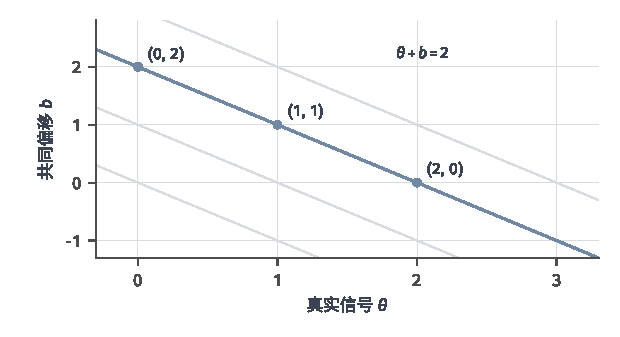
\includegraphics[width=105mm]{figures/00-shared/mathematical-preliminaries-lower/01-random-variables-distributions-and-causality/matplotlib/probability-common-bias-identification/figure.pdf}
  \caption{共同偏移模型中的等价参数。模型为\(Y_i=\theta+b+\varepsilon_i\)，\(\varepsilon_i\)相互独立且服从\(\mathcal N(0,1)\)。蓝线上的参数均满足\(\theta+b=2\)，三个标记点\((0,2),(1,1),(2,0)\)产生相同的任意样本量观测联合分布；浅灰线仅辅助比较其他参数和。}
  \label{fig:probability-common-bias-identification}
\end{figure}

不可识别还直接限制任何估计程序。对赋范目标空间，若在每个允许的样本量\(n\)下都有
\(P_{\vartheta_1}^{(n)}=P_{\vartheta_2}^{(n)}\)，但
\(\tau(\vartheta_1)\neq\tau(\vartheta_2)\)，取两目标值距离的三分之一为
\(\epsilon>0\)。任何只依赖样本的估计量\(\widehat\tau_n\)在两种机制下具有相同
分布，因而不可能同时满足
\[
  \mathbb{P}_{\vartheta_j}
  \left\{\lVert\widehat\tau_n-\tau(\vartheta_j)\rVert<\epsilon\right\}
  \longrightarrow1,\qquad j=1,2.
\]
因为两个半径为\(\epsilon\)的球不相交，同一个估计量分布不可能把趋近于一的概率
同时赋给它们。这证明了：不可识别目标不能靠增加同类样本在全部等价机制下一致恢复。

\subsection{抽样与观测机制下的识别条件}
\subsubsection{抽样制度与目标总体}
\label{sec:statistics-sampling-population}
\label{sec:statistics-missingness-observation}
% Baseline T:127-251
统计结论必须先回答“想对谁成立”。\term{目标总体}（target population）是推断希望
覆盖的对象、时间和条件的集合；\term{抽样制度}（sampling regime）描述观测如何从
这些对象产生。若样本只来自工作日的一个传感器，模型本身不能把结论自动推广到周末或
另一批设备。

独立同分布抽样把每个\(Y_i\)视为来自同一分布的独立重复。配对抽样则把
\((Y_{i,A},Y_{i,B})\)视为一个单位，例如同一对象在两种条件下的读数。若这些配对单位跨\(i\)独立，差值
\(D_i=Y_{i,A}-Y_{i,B}\)也跨\(i\)独立；把两列拆成\(2n\)个独立记录会丢失配对信息。
分层抽样预先按群组分别抽取，成组抽样则一次抽取整个设备、班级或用户群。两者的
独立单位和加权方式不同。

\paragraph{条件分母、相关性与信息量}
配对的收益取决于对内协方差：
\[
  \operatorname{Var}(D_i)
  =\operatorname{Var}(Y_{i,A})+\operatorname{Var}(Y_{i,B})
   -2\operatorname{Cov}(Y_{i,A},Y_{i,B}).
\]
正协方差会降低差值方差，负协方差则可能使配对更差；“同一对象测两次”本身并不保证
精度提高。

设目标总体中群组\(g\)的比例为\(\pi_g\)，群组均值为\(\mu_g\)，则总体均值为
\[
  \mu=\sum_g\pi_g\mu_g.
\]
总体指标可能很好，却掩盖某个小群组的严重误差。若群组中有\(n_g\)个独立Bernoulli
结果，样本比率\(\widehat p_g\)的方差为
\[
  \operatorname{Var}(\widehat p_g)
  =\frac{p_g(1-p_g)}{n_g}.
\]
这里把\(n_g\)视为固定正整数。若观测对\((G_i,Y_i)\)独立同分布，且\(Y_i\mid G_i=g\)服从Bernoulli规律，群组样本数
\(N_g=\sum_i\mathbb{I}\{G_i=g\}\)也是随机的，则
\(\widehat p_g\)只在\(N_g>0\)时有定义，且上述方差是给定\(N_g\)后的条件方差；
无条件误差还要平均随机分母，并处理\(N_g=0\)事件。不确定性由实际相关分母决定，
而不是总样本量\(n\)。报告群组公平性或来源质量时，应同时报告分母、抽样方式和区间，
不能只排列百分比。

已知入样概率时，权重可以把抽样分布重新接回目标总体。令\(S\in\{0,1\}\)表示一个
总体对象是否入样，\(\rho(Z)=\mathbb{P}(S=1\mid Z)\)，并假设
\(S\mathrel{\perp}Y\mid Z\)、\(\rho(Z)>0\)以及
\(\mathbb{E}[|Y|/\rho(Z)]<\infty\)。条件期望给出
\[
  \mathbb{E}\left[\frac{SY}{\rho(Z)}\right]
  =\mathbb{E}\left[
    \frac{\mathbb{E}[S\mid Y,Z]Y}{\rho(Z)}
  \right]
  =\mathbb{E}[Y].
\]
这条逆概率恒等式恢复的是明确的总体平均。若某一区域\(\rho(Z)=0\)，或者入样在给定
\(Z\)后仍依赖未观测的\(Y\)，等式便不能仅由已记录部分的分布推出。

记录数也不等于独立信息量。若同一来源复制一条记录十次，样本平均的显示分母增大，
实际信息却没有增加。时间序列中的相邻读数可能共享漂移；群组内记录可能共享设备偏差。
这类依赖应通过按群组建模、块抽样或
\BookSectionRef{sec:stoch-markov-long-run-average}{第~\ref{sec:stoch-markov-long-run-average}节}的相关过程工具处理，而不能
继续套用独立样本方差。

时间抽样还会改变目标本身。若传感器每分钟记录一次，朴素平均直接对应的是当天这组分钟网格时刻的平均读数。若目标是全天连续均匀时刻的平均，有限网格还只是积分近似；网格逐渐变细且读数路径可作Riemann积分时，等间隔平均才逼近该目标。若只在告警后加密采样，朴素平均通常会过度代表异常时段。
一种修正方式是记录每个目标时段被抽中的概率并作逆概率加权，但这要求这些时段都有正的入样概率。完全未覆盖的夜间时段不能靠增大已有权重恢复。抽样日志因此也属于推断所需的观测记录。

抽样制度与分析单位应在看结果前确定。假设十台设备各产生一千条记录，而处理实际随机
分配给设备，那么有效随机化单位是十台设备，不是一万条记录。记录内噪声可以帮助估计
每台设备的均值，却不能把处理效应的独立单位扩充到一万。这个区别会同时影响标准误、
置换方式和训练测试划分。

\subsubsection{缺失与选择下的目标恢复}

不完整观测带来另一类问题。令\(R=1\)表示\(Y\)被观察到，\(X\)为始终可见变量。
若高读数更容易被漏记，仅分析留下的记录就会低估总体温度。要判断观测子样本能否用于原目标，需说明缺失是否与完整数据有关，或者这种关系能否被始终可见的协变量解释。下面三种机制正是按这一依赖是否存在、能否由已见信息消除来区分。
\term{完全随机缺失}（missing completely at random, MCAR）要求
\[
  R\mathrel{\perp}(X,Y).
\]
\term{随机缺失}（missing at random, MAR）要求
\[
  R\mathrel{\perp}Y\mid X,
\]
即给定已观测协变量后，缺失概率不再依赖缺失值本身。
\term{非随机缺失}（missing not at random, MNAR）则允许这种剩余依赖。

多个变量可能按不同模式缺失，此时“已观测变量”随模式改变，不能用一个固定条件集概括全部MAR要求。
\begin{definition}[观测模式与缺失机制]
  \label{def:statistics-missingness}
  设完整数据为\(\bm Z=(Z_1,\ldots,Z_d)\)，观测指示\(\bm R\in\{0,1\}^d\)。对每种模式\(\bm r\)，定义
  \[
    O(\bm r)=\{j:r_j=1\},\qquad M(\bm r)=\{j:r_j=0\}.
  \]
  实际记录为\((\bm r,\bm Z_{O(\bm r)})\)。令\(g(\bm r\mid\bm z)\)为给定完整数据时的模式概率核。若对每种\(\bm r\)都存在只依赖已见坐标的可测函数\(g_{\bm r}\)，使
  \[
    g(\bm r\mid\bm z)=g_{\bm r}(\bm z_{O(\bm r)})
  \]
  对完整数据分布几乎处处成立，则称机制为MAR。若\(g(\bm r\mid\bm z)\)对全部模式均不依赖\(\bm z\)，则为MCAR；若MAR条件失败，则为MNAR。
\end{definition}
例如在二维数据中，模式\((1,0)\)的出现概率可依赖\(Z_1\)，却不能依赖未见的\(Z_2\)；模式\((0,1)\)反过来可以依赖\(Z_2\)，却不能依赖\(Z_1\)。这是对每种模式分别施加的条件，不能只在当前观测到的某一模式上核对。“随机缺失”也不等于“缺失标记完全随机”，后者对应更强的MCAR。

当\(\mathbb{P}(R=1)>0\)时，MCAR下完整案例仍代表总体，但效率降低。MAR下可建模
\(\mathbb{P}(R=1\mid X)\)并加权，或建模\(Y\mid X\)后插补；两者都依赖模型和
正值条件。MNAR下的目标通常不能只由已记录部分的分布识别，需要机制假设、外部信息或敏感性分析。
MAR描述的是缺失概率依赖哪些变量，并不意味着可以丢弃所有不完整记录。
“缺失机制可忽略”则要指定在哪一种推断计算中省去机制项；定义似然后，
式~\eqref{eq:statistics-missing-likelihood}将说明这种省略还需要哪些参数条件。
数据表中的一个缺失标记本身不能证明属于哪种机制。

识别障碍在有界结果上已经出现。若\(0\leq Y\leq1\)且
\(\mathbb{P}(R=0)>0\)，观测数据只给出已见部分的\(RY\)与缺失指示；把所有未见
\(Y\)设为\(0\)或设为\(1\)会产生相同观测，却给出不同总体均值。因此不加机制条件
时只能得到
\[
  \mathbb{E}[RY]
  \leq\mathbb{E}[Y]
  \leq\mathbb{E}[RY]+\mathbb{P}(R=0).
\]
两个端点分别可由把全部未见结果设为\(0\)或\(1\)达到，所以仅凭上述信息不能继续
收紧。若MAR成立，并令
\(\pi(X)=\mathbb{P}(R=1\mid X)>0\)，则第
~\ref{sec:statistics-sampling-population}节的逆概率恒等式在这里化为
\[
  \mathbb{E}\left[\frac{RY}{\pi(X)}\right]
  =\mathbb{E}[Y].
\]
正值条件负责覆盖，条件独立负责把未见结果接回已见结果；权重很大时，即使目标可识别，
有限样本方差仍可能很高。
\begin{example}[贯穿本章的传感器校准数据]
\label{ex:statistics-running-sensor-calibration}
考虑教学构造的\(25\)个独立传感器响应，暂以高斯位置模型描述，单次噪声标准差已知为
\(\sigma=2\)，样本汇总为
\[
\overline y=10.4,\qquad
\frac1{25}\sum_{i=1}^{25}(y_i-\overline y)^2=4.
\]
若另问响应如何随校准输入\(x\)变化，靠近左边界\(x_0=0\)的三个观测为
\[
(x_i,y_i)=(0,9),(1,11),(3,13),
\]
在给定带宽下核权重为\(1,0.75,0.25\)。后面的局部回归、Bootstrap、区间与预测复用这些输入，只改变所报告的目标。它们是可核算的教学数值，不是实测性能报告；把局部输入关系加入模型时，也不再把全部读数视为同一位置分布的重复抽取。
\end{example}

\section{参数与函数的估计}
\label{sec:stats-parameter-inference-efficiency}
目标能够由观测规律确定后，有限记录仍只提供它的近似。估计一个均值时，输出是一个数；估计分布或条件函数时，输出是一整条规律。两种输出都可以采用参数化或非参数化构造：样本平均无须预设分布族，完整的高斯分布却可以由均值和方差确定。下面按输出对象展开，再说明似然、矩、损失与先验如何产生估计规则。

\subsection{有限维目标的估计}
\subsubsection{基于似然的参数估计}
\label{sec:statistics-likelihood-robustness}
\label{sec:statistics-bayes-hierarchy}
% Baseline T:266-439
同一组已见记录可以放在不同候选参数下评价：模型在这些记录处的概率质量或密度有多大？保持数据不变、让候选参数变化，就得到拟合所需的比较函数。它使用的是观测模型的质量或密度，而不是给参数直接分配概率。
给定观测\(\bm{y}\)后，\term{似然}（likelihood）
\[
  L(\vartheta;\bm{y})=p_\vartheta(\bm{y})
\]
相对于模型共同的参考测度定义，把数据固定，把参数看作待比较的变量。似然不是参数的
概率分布；只有再指定先验并归一化后，才得到后验分布。最大似然估计选择
\(\widehat\vartheta_{\mathrm{MLE}}\in\argmax_\vartheta L(\vartheta;\bm{y})\)，
通常等价于最小化负对数似然\scite{vanderVaart1998asymptotic}。

现在可以明确前面的缺失机制可忽略性。以连续数据为例，令\(p_\theta\)描述完整数据，
\(g_\psi\)描述缺失模式；\(\theta\)与\(\psi\)分别是两者的参数。若整个模型满足MAR，
固定已见模式\(\bm r\)与坐标\(\bm z_{\mathrm{obs}}\)后，观测似然分解为
\begin{equation}
\begin{aligned}
 L_{\mathrm{obs}}(\theta,\psi)
 &=\int p_\theta(\bm z_{\mathrm{obs}},\bm z_{\mathrm{mis}})
       g_\psi(\bm r\mid\bm z_{\mathrm{obs}})\,\mathrm d\bm z_{\mathrm{mis}}\\
 &=g_\psi(\bm r\mid\bm z_{\mathrm{obs}})
       L_{\mathrm{data}}(\theta),\\
 L_{\mathrm{data}}(\theta)
 &=\int p_\theta(\bm z_{\mathrm{obs}},\bm z_{\mathrm{mis}})
       \,\mathrm d\bm z_{\mathrm{mis}}.
\end{aligned}
\label{eq:statistics-missing-likelihood}
\end{equation}
离散坐标把相应积分换成求和。若参数域是直积\(\Theta\times\Psi\)，即两组参数可独立变化，
在机制因子为正的观测上比较\(\theta\)的似然时便可省去这个不含\(\theta\)的因子。
这里省去的是机制模型的计算，保留的是对缺失坐标积分后的数据似然；直接删除不完整行
不是这项分解允许的操作。

用两个二元坐标可以把这一步算完。设每行的两个坐标独立同分布，
\(Z_{i1},Z_{i2}\sim\operatorname{Bernoulli}(\theta)\)，
第一列总被记录，第二列是否缺失只取决于第一列，因而机制不依赖缺失值本身，
满足MAR。按第二列求和后，观测似然成为
\[
  L_{\mathrm{obs}}(\theta,\psi)
  =g_\psi(\bm r\mid \bm z_{\mathrm{obs}})
   \prod_i\Bigl[\theta^{z_{i1}}(1-\theta)^{1-z_{i1}}\Bigr].
\]
机制因子不含\(\theta\)，所以比较\(\theta\)时可以略去它；
剩下的是对每一行第一列的似然，第二列缺失的行同样参与。
这正是“对缺失坐标积分”与“丢掉整行”的差别：前者保留了第一列的信息，
后者把它们一并舍弃，估计量一般不再无偏。
若缺失机制反过来依赖第二列自身的取值，上述分解失效，
仅用已见数据不足以恢复\(\theta\)，需要显式写出机制模型。

对\(Y_i\overset{\mathrm{iid}}{\sim}\mathcal{N}(\theta,\sigma^2)\)，且
\(\sigma^2>0\)已知，
\[
  -\log L(\theta;\bm{y})
  =\frac{1}{2\sigma^2}\sum_{i=1}^n(y_i-\theta)^2+C.
\]
对\(\theta\)求导并令其为零，得到
\(\widehat\theta=\overline y\)。同一个样本平均也可由矩估计得到：总体矩
\(\mathbb{E}_\theta[Y]=\theta\)，于是令样本矩\(\overline Y\)等于总体矩。
似然法依赖完整分布形式，矩估计只使用选定矩条件。

“令导数为零”只寻找内点候选，不保证最大值存在或唯一。例如独立Bernoulli观测的
似然为
\[
  L(p;\bm y)=p^{\sum_i y_i}(1-p)^{n-\sum_i y_i},\qquad p\in[0,1].
\]
当样本同时含有\(0\)和\(1\)时，唯一最大值是样本比例；全为\(1\)或全为\(0\)时，
最大值分别落在边界\(p=1\)或\(p=0\)。若错误地把参数域写成开区间\((0,1)\)，
边界数据甚至只有上确界而没有最大似然估计。

压缩数据会丢掉细节，但有时这些细节与目标参数无关。例如Bernoulli样本的排列不同，只要成功次数相同，似然关于\(p\)的依赖就相同。充分性要求这种“保留全部参数信息”在整个指定模型中成立。
\begin{definition}[充分统计量]
  \label{def:statistics-sufficient-statistic}
  设样本\(\bm Y\)与统计量\(T(\bm Y)\)取值于标准Borel空间。若存在概率核\(K(t,\cdot)\)，对每个\(\vartheta\in\Theta\)都是\(\bm Y\)给定\(T=t\)的正则条件分布版本，而且\(K\)不依赖\(\vartheta\)，则称\(T\)为该模型的\term{充分统计量}（sufficient statistic）。各条件分布的等式按相应\(P_\vartheta^T\)-几乎处处意义理解。
\end{definition}
它是在给定摘要后，样本其余部分不再携带关于参数的信息。在受同一个\(\sigma\)有限测度支配的模型中，若密度可分解为
\[
  p_\vartheta(\bm y)=g_\vartheta(T(\bm y))h(\bm y),
\]
则因子分解定理说明\(T\)对\(\vartheta\)充分。直观地说，给定
\(T(\bm Y)=t\)后，条件密度中的参数因子在归一化时抵消，剩余分布不含
\(\vartheta\)。在有限离散样本空间上，逆向关系也可直接算出。若
\(\bm Y\mid T=t\)的条件质量\(k(\bm y\mid t)\)不依赖参数，则
\[
  p_\vartheta(\bm y)
  =p_\vartheta^T(T(\bm y))k(\bm y\mid T(\bm y)),
\]
也得到所需分解。一般连续情形的条件分布可能集中在低维纤维上，不能把这个离散乘法式未经参考测度核对就当成普通密度恒等式；因子分解定理负责一般受支配模型中的等价性。高斯位置模型中，已知方差时
\(\sum_iY_i\)充分。充分性是相对于指定模型而言的；模型失配后，压缩掉的部分可能正好
暴露失配。

\subsubsection{基于经验准则的估计与稳健性}
似然以指定模型的对数密度作为拟合准则。若目标是中位数、希望减轻异常值影响，或不愿假定完整分布形状，就需要按目标另选样本准则。下面的表达把这些估计方法放在同一个框架中，但不同准则的总体最小点未必相同。
\begin{definition}[M估计]
  \label{def:statistics-m-estimator}
给定可测准则\(\rho(y,\vartheta)\)，当下面的最小点集合非空且存在可测选择时，\term{\(M\)估计}（M-estimation）是从中选出的一个可测统计量：
\[
  \widehat\vartheta
  \in\argmin_{\vartheta\in\Theta}
  \frac1n\sum_{i=1}^n\rho(Y_i,\vartheta).
\]
\end{definition}
准则可微且最优点位于参数域内点时，一阶必要条件是估计方程
\[
  \frac1n\sum_{i=1}^n\psi(Y_i,\widehat\vartheta)=0,
  \qquad
  \psi(y,\vartheta)=\nabla_\vartheta\rho(y,\vartheta).
\]
取平方准则\(\rho(y,\theta)=(y-\theta)^2/2\)，就有\(\psi(y,\theta)=\theta-y\)，每个残差的作用随绝对值线性增长。
若\(\mathbb E|Y|<\infty\)，绝对损失\(\rho(y,\theta)=|y-\theta|\)的总体风险有限，
其最小点则是中位数：目标函数的左右
方向导数分别由\(\mathbb{P}(Y<\theta)\)与\(\mathbb{P}(Y>\theta)\)决定，最优条件是
\(\mathbb{P}(Y\leq\theta)\geq1/2\)且
\(\mathbb{P}(Y\geq\theta)\geq1/2\)。因此平方与绝对准则即使使用同一批位置数据，
也在估计不同的总体泛函。

\(M\)估计的一致性需要把经验准则与总体准则连接起来。记
\[
  Q_n(\vartheta)=\frac1n\sum_{i=1}^n\rho(Y_i,\vartheta),
  \qquad
  Q(\vartheta)=\mathbb{E}[\rho(Y,\vartheta)].
\]
设\(Q\)有限，并在唯一点\(\vartheta^\star\)取得最小值，并且该最小值
分离，即对每个\(\epsilon>0\)，
\[
  \inf_{\lVert\vartheta-\vartheta^\star\rVert\geq\epsilon}
  Q(\vartheta)>Q(\vartheta^\star).
\]
若\(\sup_{\vartheta\in\Theta}|Q_n(\vartheta)-Q(\vartheta)|
\xrightarrow{\mathbb{P}}0\)，且近似优化误差
\[
  Q_n(\widehat\vartheta_n)-\inf_{\vartheta\in\Theta}Q_n(\vartheta)
  =o_{\mathbb{P}}(1),
\]
其中\(o_{\mathbb{P}}(1)\)表示该随机误差依概率趋于零，则
\(\widehat\vartheta_n\xrightarrow{\mathbb{P}}\vartheta^\star\)。证明只需比较准则：
在任意固定的\(\epsilon\)球外，总体准则有正间隔；当一致偏差和优化误差都小于该
间隔的适当分数时，经验近似最小点不可能位于球外。这里使用全参数域上的一致偏差和球外分离，不另需紧性。若只能在紧集上证明一致收敛，就还需控制估计点落在这些紧集之外的概率。总体最小点不唯一时，可在相应的集合分离条件下研究估计点到最小点集合的距离。

若真实分布\(P_0\)不属于\(\mathcal P\)，就不能把拟合参数直接解释为真实机制的参数。其总体对数损失目标是：
\begin{definition}[伪真参数]
  \label{def:statistics-pseudo-true-parameter}
相对于共同参考测度的模型密度\(p_\vartheta\)，假定所比较的\(\mathbb E_{P_0}\log p_\vartheta(Y)\)均有定义，且下列最大点集合非空。集合中的任一点
\[
  \vartheta^\star
  \in\argmax_\vartheta\mathbb{E}_{P_0}[\log p_\vartheta(Y)]
\]
称为该准则的\term{伪真参数}（pseudo-true parameter）。
\end{definition}
在经验准则一致逼近、总体极值唯一且分离等条件下，最大似然估计才趋向该点；多个最大点时须改为集合结论。它是模型族中按对数损失最接近
真实分布的点，不必等于科学问题中的真实量。估计量收敛并不自动证明模型正确。

\paragraph{稳健损失与影响函数}
为了限制异常残差的作用，可使用阈值\(c>0\)的Huber损失
\[
  \rho_c(r)=
  \begin{cases}
    r^2/2,& |r|\leq c,\\
    c|r|-c^2/2,& |r|>c,
  \end{cases}
  \qquad
  \psi_c(r)=
  \begin{cases}
    r,& |r|\leq c,\\
    c\operatorname{sign}(r),& |r|>c.
  \end{cases}
\]
这里\(\psi_c(r)=\rho_c'(r)\)是损失对残差\(r\)的导数。由于
\(\nabla_\theta\rho_c(y-\theta)=-\psi_c(y-\theta)\)，位置估计的参数梯度方程
整体乘以\(-1\)后，等价地写成
\(\sum_i\psi_c(y_i-\widehat\theta)=0\)。小残差仍按平方损失处理，大残差的贡献被截在
\(\pm c\)。代价是：即使高斯模型完全正确，较小的\(c\)也会舍弃一部分有效幅度信息。

总体准则确定估计目标，却没有说明少量异常观测会把它拉动多少。可以向分布\(P\)加入比例为\(\epsilon\)的单点污染，再考察目标的一阶变化。
\begin{definition}[影响函数]
  \label{def:statistics-influence-function}
  设\(T\)为定义在概率分布上的实值或向量值统计泛函，\(\Delta_z\)为全部质量集中在\(z\)的概率测度。假定充分小的正\(\epsilon\)所对应的污染分布仍在\(T\)的定义域内；若右侧极限存在且有限，定义\term{影响函数}（influence function）为
  \[ \operatorname{IF}(z;T,P)=\lim_{\epsilon\downarrow0}
    \frac{T((1-\epsilon)P+\epsilon\Delta_z)-T(P)}{\epsilon}. \]
\end{definition}
例如对均值泛函，\(\operatorname{IF}(z;T,P)=z-\mathbb E_PY\)：同样少量的污染，位置越远，拉动越大。下面先用标量估计方程说明这项敏感性。设统计泛函
\(T(P)\)由
\[
  \mathbb{E}_P[\psi(Y,T(P))]=0
\]
定义，并令\(P_\epsilon=(1-\epsilon)P+\epsilon\Delta_z\)。记
\(A=\mathbb{E}_P[\partial_\theta\psi(Y,T(P))]\neq0\)。假设估计方程在
\(\epsilon=0\)附近可微，微分可移入期望，且所跟踪的根在局部唯一。对
\(\mathbb{E}_{P_\epsilon}[\psi(Y,T(P_\epsilon))]=0\)在
\(\epsilon=0\)处隐式求导，得到
\[
  0=-\mathbb{E}_P[\psi(Y,T(P))]
    +\psi(z,T(P))+A\,T'(0),
\]
第一项为零，因此
\begin{equation}
  \operatorname{IF}(z;T,P)=T'(0)
  =-A^{-1}\psi(z,T(P)).
  \label{eq:statistics-influence-function}
\end{equation}
平方损失的位置影响随\(z\)无界，Huber得分则有界。多维参数时\(A\)是估计方程的
Jacobian矩阵，式~\eqref{eq:statistics-influence-function}要求该矩阵可逆；经验风险中它常表现为Hessian矩阵近似，但只有可微、局部可逆且估计根稳定时，
这种近似才成立。影响函数只描述污染比例在零附近的一阶敏感性，不是任意污染比例下的
误差上界；在回归中，截断残差也不会自动限制极端输入产生的高杠杆影响。

图~\ref{fig:statistics-huber-loss}区分损失本身与它的导数。大残差的Huber损失仍持续增加，并不是把异常观测删除；被限制的是单个残差进入位置估计方程的得分。把“损失增长较慢”直接说成“整个估计量的影响有界”，还需要式~\eqref{eq:statistics-influence-function}中的局部曲率与输入条件。

\begin{figure*}[htbp]
  \centering
  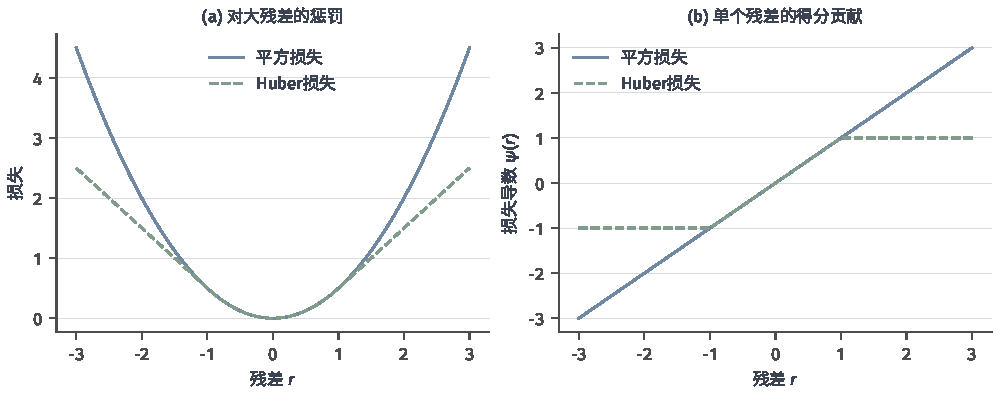
\includegraphics[width=\linewidth]{figures/00-shared/mathematical-preliminaries-lower/01-random-variables-distributions-and-causality/matplotlib/statistics-huber-loss/figure.pdf}
  \caption{平方损失与阈值\(c=1\)的Huber损失（解析式教学图）。左图比较惩罚值，右图比较对残差的导数；Huber得分在\([-1,1]\)内截断。横轴是构造残差，不代表实测异常值分布。}
  \label{fig:statistics-huber-loss}
\end{figure*}
\paragraph{污染模型与中位数的稳定性}
限制异常值影响之前，要先说明允许观测规律偏离到什么范围。常见的污染模型写成
\[
 P_\epsilon=(1-\epsilon)P_0+\epsilon Q,\qquad 0\leq\epsilon<1,
\]
其中\(P_0\)是希望拟合的主体规律，\(Q\)可为任意污染分布。目标若是\(P_0\)的位置参数，不能把\(P_\epsilon\)的均值自动当成该参数：即使污染比例很小，\(Q\)的尾部也能使均值偏移任意远，甚至不再存在。稳健准则必须同时说明希望保留的目标、允许的污染和所控制的误差\scite{huber1964}。

样本中位数能直接说明一种有限样本稳定性。取奇数个读数\(n=2k+1\)，把第\(k+1\)个顺序统计量作为中位数。若至多\(k\)条读数被任意替换，仍有至少\(k+1\)条未污染记录，因此中位数一定落在未污染读数的最小值与最大值之间：落在左侧或右侧都需要至少\(k+1\)条记录越过这个范围。替换\(k+1\)条则可把中位数推到任意远。对这个奇数样本约定，使估计值可以无界偏移的最小替换比例为\((k+1)/(2k+1)\)，趋近于\(1/2\)；均值只需替换一条，比例为\(1/n\)。这里讨论的是替换失效阈值，不是中位数对原位置参数的误差一定很小。

把同一计算用于局部窗口，就得到窗口中位数滤波。例如五个邻近读数为\((10,11,9,10,1000)\)，均值为\(208\)，中位数为\(10\)。这种收益依赖窗口内的主体值确实应当相近；窄峰、细线或边界附近的真实结构也可能被当作少数值抹去。它控制单个窗口内的排序敏感性，并不使相邻窗口输出独立。

\paragraph{基于最小子集的稳健模型拟合}
在直线或几何变换拟合中，异常匹配还可能具有极端输入位置，仅截断残差不能自动消除高杠杆影响。随机抽样一致性（random sample consensus, RANSAC）反复抽取足以确定模型的最小子集，生成候选参数，按预先指定的残差阈值找出相容记录，再用相容集重新拟合\scite{vision-ransac-1981}。阈值、最小子集大小和模型可识别性共同决定何种记录可算相容。

设每次随机抽样全为内点且能产生有效候选的概率至少为\(q\in(0,1)\)，不同轮次独立，连续\(K\)轮都未抽到这种子集的概率至多为\((1-q)^K\)。要求该失败概率不超过\(\delta\in(0,1)\)，足够取
\begin{equation}
 K\geq\left\lceil\frac{\log\delta}{\log(1-q)}\right\rceil.
 \label{eq:statistics-ransac-trials}
\end{equation}
若子集含\(m\)条独立内点标记、内点概率为\(w\)，且全内点子集总能确定有效模型，则\(q=w^m\)。从固定的\(n\)条记录中无放回抽取\(m\)条时，全内点概率应改为\(\binom{n_{\rm in}}m/\binom nm\)，其中\(n_{\rm in}\geq m\)；退化配置还会进一步降低有效概率。例如取独立标记模型的\(w=1/2,m=2,\delta=0.01\)，需\(K\geq17\)轮。

这个界只控制是否抽到有效内点子集。若阈值过宽、错误结构具有更大相容集，或全内点仍不能唯一确定模型，最终选择仍可能错误。用当前最大相容集的比例代替未知\(w\)只能得到依赖估计的停止规则，不能未经额外论证继续宣称上述确定概率保证。

\subsubsection{后验推断与层次汇聚}
% Baseline T:750-783
点估计只报告一个候选值，没有保留其他候选参数的不确定性。这个值可以是估计均值、中位数或其他目标的结果，不统一表示密度最大的参数位置。若还希望把已有的参数不确定性与新观测记录合在一起，可以先在候选参数上指定一张概率分布，再按各参数对这些记录的似然重新加权。Bayes更新沿这条路线产生参数的条件分布，所用先验是额外的建模条件。
频率学派把参数固定而把样本看作随机。Bayes方法另给参数指定先验
\(\pi(\theta)\)，观测后用
\[
  \pi(\theta\mid\bm y)
  =
  \frac{p(\bm y\mid\theta)\pi(\theta)}
       {\int p(\bm y\mid u)\pi(u)\,\mathrm du}
\]
得到\term{后验分布}（posterior distribution）。它把似然提供的数据证据与先验
假设合并。这个公式要求分母，即模型证据，严格为正且有限；否则右侧不能定义概率分布。

对式~\eqref{eq:statistics-missing-likelihood}中的两组参数，若先验还满足
\(\pi(\theta,\psi)=\pi_\Theta(\theta)\pi_\Psi(\psi)\)，则联合后验的未归一化密度分成
\[
 \{L_{\mathrm{data}}(\theta)\pi_\Theta(\theta)\}
 \{g_\psi(\bm r\mid\bm z_{\mathrm{obs}})\pi_\Psi(\psi)\}.
\]
在归一化常数严格为正且有限时，对\(\psi\)积分只产生与\(\theta\)无关的常数，
所以关于\(\theta\)的后验也可省去机制因子。这就是Bayes分析还需要先验可分离的含义；
若先验把两组参数联系起来，该因子一般会通过\(\psi\)影响\(\theta\)的后验\scite{pgm-parameter-learning-rubin1976}。

后验二阶矩有限时，后验均值最小化后验平方损失。事实上，对任意行动\(a\)，令
\(m=\mathbb{E}[\theta\mid\bm y]\)，则
\[
  \mathbb{E}[(\theta-a)^2\mid\bm y]
  =\operatorname{Var}(\theta\mid\bm y)+(a-m)^2.
\]
后验一阶绝对矩有限时，后验中位数则最小化后验绝对损失，其理由与前文总体中位数的左右方向导数相同。最大后验
估计只选择相对于指定参考测度的密度峰值；非线性重参数化会引入Jacobian因子，因此峰值
位置一般不保持不变。三种Bayes行动不必相同。

设
\[
  Y_i\mid\theta\overset{\mathrm{iid}}{\sim}\mathcal N(\theta,\sigma^2),
  \qquad
  \theta\sim\mathcal N(\mu_0,\tau_0^2).
\]
取\(\sigma^2,\tau_0^2>0\)。配方后得到共轭更新
\[
  \theta\mid\bm y
  \sim\mathcal N(\mu_n,\tau_n^2),\qquad
  \tau_n^{-2}=\tau_0^{-2}+n\sigma^{-2},
\]
\[
  \mu_n=\tau_n^2
  \left(\frac{\mu_0}{\tau_0^2}+\frac{n\overline y}{\sigma^2}\right).
\]
后验均值是先验均值与样本均值按精度加权的折中。新读数的后验预测还须加上观测噪声，见第~\ref{sec:statistics-scoring-calibration}节。
% Baseline T:792-834

离散比例也有同样的共轭结构。若
\(Y_i\mid p\overset{\mathrm{iid}}{\sim}\operatorname{Bernoulli}(p)\)且
\(p\sim\operatorname{Beta}(a,b)\)，观察到\(s=\sum_iY_i\)个成功后，
\[
  p\mid\bm y\sim\operatorname{Beta}(a+s,b+n-s).
\]
对\(K\)类计数\((n_1,\ldots,n_K)\)，Dirichlet先验
\(\operatorname{Dirichlet}(\alpha_1,\ldots,\alpha_K)\)相应更新为
\(\operatorname{Dirichlet}(\alpha_1+n_1,\ldots,\alpha_K+n_K)\)。这些更新依赖
给定比例后的条件独立抽样；过度离散或来源相关时，简单加计数会夸大信息量。

\paragraph{层次模型与部分汇聚}
多个设备、标注者或任务的数据量很不均衡时，可令
\[
  \theta_g\mid\mu,\tau^2\sim\mathcal N(\mu,\tau^2),\qquad
  Y_{g,i}\mid\theta_g\sim\mathcal N(\theta_g,\sigma_g^2).
\]
这里假设给定\((\mu,\tau^2)\)后各组参数\(\theta_g\)条件独立，并且给定全部组参数后，
所有\(Y_{g,i}\)也条件独立。若\(\mu,\tau^2,\sigma_g^2\)暂视为已知，\(\tau^2,\sigma_g^2>0\)，且第\(g\)组有
\(n_g\geq1\)个观测，则
\[
  \theta_g\mid\bm y_g,\mu,\tau^2
  \sim\mathcal N(m_g,V_g),\qquad
  V_g^{-1}=\tau^{-2}+n_g\sigma_g^{-2},
\]
\[
  m_g
  =V_g\left(\frac{\mu}{\tau^2}
    +\frac{n_g\overline y_g}{\sigma_g^2}\right).
\]
固定超参数时，第\(g\)组后验只依赖\(\bm y_g\)以及外部给定的共同中心和尺度；
小样本群组会更强地向共同中心\(\mu\)收缩，其他组数据尚未进入该后验。
当用全部群组数据估计共同超参数，或在完整Bayes模型中对其后验积分时，其他组数据才会
通过共同超参数间接改变第\(g\)组的推断，从而形成组间信息共享。
\(\tau^2\to0\)接近完全汇聚，\(\tau^2\to\infty\)接近各组独立估计，有限正尺度给出
部分汇聚。若超参数由同一数据估计，这是经验Bayes；若继续给它们指定先验，推断对象还
包括超参数后验。
这不是免费增加数据，而是加入“群组来自共同总体”的结构假设。若群组机制不同或先验
尺度过窄，收缩会掩盖真实差异。先验由研究者指定并不把固定物理参数变成随机生成的
事实；Bayes概率表达的是模型内部的不确定性。

有限维推断的目标也可以是一组总体分位数。设\(Y_1,\ldots,Y_n\)独立同分布且\(0<q<1\)，经验分布
\(\widehat F_n(y)=n^{-1}\sum_i\mathbb I_{\{Y_i\leq y\}}\)的广义逆给出
\(\widehat q=Y_{(\lceil nq\rceil)}\)。它估计的是总体分位数，不是未来读数的覆盖阈值；后者在共形预测中使用不同的秩修正。若总体在目标分位附近严格越过水平\(q\)，经验分布的统一收敛保证该估计一致；平坦区间、原子与不唯一目标则需按所选分位约定分析。

\subsection{分布与条件函数的估计}
\subsubsection{经验分布与密度估计}
\label{sec:statistics-nonparametric-missing}
经验分布把每个样本点赋质量\(1/n\)，因而是完整的概率分布而不是密度曲线。独立同分布样本下，Glivenko--Cantelli定理给出
\(\sup_y|\widehat F_n(y)-F(y)|\to0\)几乎必然；固定\(y\)的大数定律本身尚不等于这个统一结论。参数化方法则可报告\(P_{\widehat\theta}\)，例如
\(\mathcal N(\overline Y,S^2)\)，其有效性另外依赖模型限制。下面的平滑表示改变了分布或条件函数的形状，需要同时控制逼近误差与局部样本波动。
% Baseline T:1474-1583
有限维模型可能把真实分布限制得过强。非参数方法不预先固定有限个参数，但仍通过带宽、
邻域或平滑度控制复杂度。以下令\(Y_1,\ldots,Y_n\)独立同分布，具有同一个一维
密度\(f\)，并采用不依赖本批观测的带宽\(h=h_n>0\)。相关、选择或加权样本
需要另行计算期望与协方差，不能直接使用下面的独立样本公式。给定宽度为\(h\)的分箱，直方图用
“箱内样本数除以\(nh\)”作为箱内常数密度；移动箱边界可能改变估计。核密度估计则把
每个样本扩散为核：
\[
  \widehat f_h(x)
  =\frac1{nh}\sum_{i=1}^n
    K\left(\frac{x-Y_i}{h}\right).
\]
若\(K\geq0\)、积分为\(1\)，则\(\widehat f_h\)本身是非负且积分为\(1\)的密度。
为直接使用局部Taylor展开，以下采用一组充分条件：\(K\)非负、积分为\(1\)、有界、紧支撑且对称，
二阶矩记为\(\mu_2(K)=\int u^2K(u)\,\mathrm du\)，并记
\(R(K)=\int K(u)^2\,\mathrm du\)；两者均有限。设\(f\)在内部点\(x\)的邻域
二阶连续可微，则小带宽下核只涉及这个光滑邻域，由
\[
  \mathbb{E}[\widehat f_h(x)]
  =\int K(u)f(x-hu)\,\mathrm du
\]
作Taylor展开，核的一阶矩因对称性消失，从而得到
\[
  \operatorname{Bias}\{\widehat f_h(x)\}
  =\frac{h^2\mu_2(K)}2f''(x)+o(h^2),
\]
\[
  \operatorname{Var}\{\widehat f_h(x)\}
  =\frac{f(x)R(K)}{nh}+o((nh)^{-1}),
\]
其中渐近式取\(h\to0\)、\(nh\to\infty\)。较大带宽降低方差却增加平滑偏差。
边界附近因核质量落到支持集外，上述对称展开失效。
在\(d\)维中，体积因子变为\(h^d\)，代表性点态方差阶数相应为
\(1/(nh^d)\)。因此维数增加会更快消耗局部样本；一维的带宽结论不能不改条件直接
移植到高维。

\subsubsection{条件均值与分位数的估计}
这里的观测改为\((X_i,Y_i)_{i=1}^n\)，假定它们来自同一联合分布且独立同分布，
\(Y\)可积。采用前面核密度估计中的非负、有界、紧支撑核\(K\)与确定带宽\(h>0\)。
回归函数\(m(x)=\mathbb{E}[Y\mid X=x]\)可由局部平均估计；以下比值只在
权重和\(\sum_iK((X_i-x)/h)>0\)时定义：
\[
  \widehat m_h(x)=
  \frac{\sum_iK((X_i-x)/h)Y_i}
       {\sum_iK((X_i-x)/h)}.
\]
局部线性回归在\(x\)附近拟合\(a+b(X_i-x)\)，在相应平滑条件下可减轻设计
密度不均和边界偏差。下面的唯一拟合还要求局部加权设计满秩；在这个一维两参数问题中，
即正权重的输入至少含两个不同取值。若权重和为零或设计退化，需扩大邻域或另给退化处理，
不能照用比值或逆矩阵公式。
\[
  (\widehat a,\widehat b)
  \in\argmin_{a,b}\sum_{i=1}^n
  K\left(\frac{X_i-x}{h}\right)
  \{Y_i-a-b(X_i-x)\}^2,
  \qquad \widehat m_{\mathrm{local}}(x)=\widehat a.
\]
\(k\)近邻取\(1\leq k\leq n\)，用离\(x\)最近的\(k\)个样本平均；距离并列时
按预先指定的规则选择。维数增大时，为包含足够邻居必须扩大
邻域，Taylor局部性随之变差，这就是维数灾难的一种表现。

在例~\ref{ex:statistics-running-sensor-calibration}的左边界\(x_0=0\)，局部常数
估计为
\[
  \widehat m_h(0)
  =
  \frac{1\times9+0.75\times11+0.25\times13}
       {1+0.75+0.25}
  =10.25.
\]
局部线性拟合令\(u_i=x_i-x_0\)。由这三个点可算得
\[
  S_0=\sum_i w_i=2,\quad
  S_1=\sum_i w_i u_i=1.5,\quad
  S_2=\sum_i w_i u_i^2=3,
\]
\[
  T_0=\sum_i w_i y_i=20.5,\qquad
  T_1=\sum_i w_i u_i y_i=18.
\]
加权正规方程给出
\[
  \widehat a
  =\frac{S_2T_0-S_1T_1}{S_0S_2-S_1^2}
  =9.2,\qquad
  \widehat b
  =\frac{S_0T_1-S_1T_0}{S_0S_2-S_1^2}
  =1.4.
\]
因此局部线性预测为\(9.2\)，而局部常数预测为\(10.25\)。在边界处，后者只能对单侧
观测加权平均，前者还估计局部斜率并把直线截距放回\(x_0\)；哪一个更接近真实条件均值
仍取决于局部线性近似和带宽是否合适，不能由这一组数值单独决定。

图~\ref{fig:statistics-local-boundary-fit}显示这两个预测值的几何区别：水平线只改变高度，斜线同时解释输入位置与响应的局部变化，再把截距取回边界点。图中的观测和权重就是上面的三个教学数据；未画出未知的真实条件均值，因此不能从图上断言哪一种估计误差更小。
\begin{figure}[htbp]
  \centering
  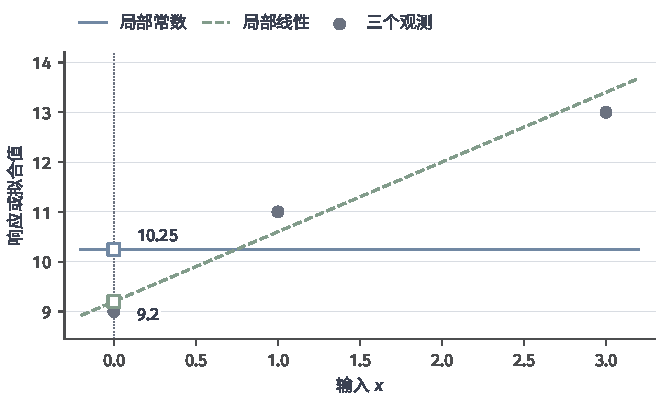
\includegraphics[width=\linewidth]{figures/00-shared/mathematical-preliminaries-lower/01-random-variables-distributions-and-causality/matplotlib/statistics-local-boundary-fit/figure.pdf}
  \caption{边界处的局部常数与局部线性拟合（教学数据图）。观测为\((0,9),(1,11),(3,13)\)，权重为\(1,0.75,0.25\)。蓝实线为加权常数\(10.25\)，绿虚线为\(9.2+1.4x\)，边界\(x_0=0\)处分别预测\(10.25\)和\(9.2\)。}
  \label{fig:statistics-local-boundary-fit}
\end{figure}

在上述独立同分布抽样下，这些方法的一致性需要邻域既缩小又包含越来越多样本。
例如一维内部点处，若输入密度在
\(x\)附近连续且为正，条件均值足够光滑，条件方差局部有界，并取
\(h\to0\)、\(nh\to\infty\)，局部常数估计的平滑偏差消失，局部平均的方差也消失。
输入密度与条件均值都二阶连续可微时，常用局部展开给出\(O(h^2)\)的平滑偏差
以及\(O((nh)^{-1})\)的方差，因此平滑偏差的平方为\(O(h^4)\)；精确常数还依赖
核、输入密度与条件噪声。近邻版本相应要求\(k\to\infty\)且\(k/n\to0\)。
这些都是目标分布有局部覆盖时的内插结论；在训练输入密度为零的区域，缩小邻域无法产生
新信息，外推保证必须来自额外结构假设。
% Baseline T:977-988
局部均值平均正负误差，不能直接给出较高的风险分位点。若报告值为\(a\)，低报时残差\(Y-a>0\)，高报时残差为负；希望估计较高分位数，就应让低报承担更大的单位代价。给定所求分位水平\(q\in(0,1)\)，下面用\(q\)与\(1-q\)分别加权这两侧绝对误差，再由左右导数核验最小点恰好满足分位数条件。
条件分位数可由\term{分位数回归}估计。假设\(Y\)可积，使下面损失的条件期望对几乎每个\(x\)有限。令
\[
  \rho_q(u)=u\bigl(q-\mathbb{I}_{\{u<0\}}\bigr),
\]
则条件\(q\)分位数最小化
\(\mathbb{E}[\rho_q(Y-a)\mid X=x]\)。固定\(x\)并记条件分布函数为\(F\)，目标对
\(a\)的次梯度区间是
\[
  [F(a^-)-q,\ F(a)-q].
\]
因此最优点恰好满足\(F(a^-)\leq q\leq F(a)\)；连续严格递增时才简化为
\(F(a)=q\)。因此分位数损失的最小点集合正是\(\mathcal Q_q\)，可能不唯一，
而\(F^{-1}(q)\)仍是其中按约定选出的单个代表。分位数回归直接估计条件分布的位置，
不要求误差为高斯或方差恒定。
实际分位数回归把条件分位函数写成\(a=f(x)\)，最小化
\(\sum_i\rho_q(Y_i-f(X_i))\)及可能的正则项。线性、样条或其他函数类限制决定了可表示的条件分位形状；最小化同一损失不意味着所有表示有同样的偏差与覆盖保证。

\section{未来观测的预测}
\label{sec:stats-prediction-observation-limits}
即使总体均值已知，下一次传感器读数仍会受新噪声影响。预测要把这种结果波动与估计未知规律的误差同时纳入。若先得到未来结果的分布，就能按所采用的损失选择报告内容：平方损失对应均值，绝对损失对应中位数，错判损失对应最可能类别；预测集合则保留一组结果并说明其覆盖概率。

\subsection{预测分布的计算与评价}
\label{sec:statistics-scoring-calibration}
若参数给定，条件预测使用概率核\(P_\theta(Y_{\rm new}\in\cdot\mid X_{\rm new}=x)\)；
代入估计得到插件预测，Bayes方法则对参数后验积分：
\[
P(Y_{\rm new}\in A\mid\bm y,x)
=\int P_\theta(Y_{\rm new}\in A\mid x)\,\pi(\mathrm d\theta\mid\bm y),
\]
这里假设给定参数后新观测与训练数据按模型条件独立。代入一个参数通常没有传播全部参数不确定性。
在前述高斯共轭模型中，
% Baseline T:784-790
\[
  Y_{n+1}\mid\bm y
  \sim\mathcal N(\mu_n,\sigma^2+\tau_n^2).
\]
其中\(\tau_n^2\)是参数不确定性，\(\sigma^2\)是新观测自身的噪声。
% Baseline T:1358-1467
点预测只给一个结果，概率预测则给出整个候选分布。若只奖励是否猜中最可能结果，报告完整概率并没有优势；评分必须鼓励把真实不确定性如实报告。
\begin{definition}[适当评分规则]
  \label{def:statistics-proper-scoring-rule}
  给定预测分布类\(\mathcal P\)，\term{评分规则}（scoring rule）\(S(Q,y)\)，即报告预测分布\(Q\)而结果为\(y\)
时承担的损失。假定所比较的期望均有定义，且诚实报告的期望有限。若对每个\(P,Q\in\mathcal P\)有\(\mathbb E_PS(P,Y)\leq\mathbb E_PS(Q,Y)\)，就称评分规则
\term{适当}（proper）；若适用分布类中的最小点唯一，则称为严格适当。
\end{definition}
它奖励诚实概率，而不是只检查最可能类别是否猜中。

对数评分的适当性直接回用第~\ref{chap:information-theory-and-statistical-geometry}章的KL散度及其非负性。下面取有限结果集\(\mathcal Y\)，用\(p,q\)表示真实分布与报告分布的概率质量函数；在真实分布赋正概率处报告零概率时，对数损失为正无穷。

离散结果的对数评分为\(S(Q,y)=-\log q(y)\)。根据上述定义，其期望差满足
\[
  \mathbb{E}_P[S(Q,Y)]-\mathbb{E}_P[S(P,Y)]
  =\sum_{y\in\mathcal Y}p(y)\log\frac{p(y)}{q(y)}
  =D_{\mathrm{KL}}(P\Vert Q)\geq0.
\]
因此对数评分是严格适当的；零预测概率遗漏真实分布的支持时，期望损失为无穷。
连续密度版本还要求相对于共同参考测度定义密度，并保证相关对数期望有定义；改变参考
坐标会改变单个对数密度值，但在合法换元下比较同一结果分布的期望差保持一致。

二元结果\(Y\in\{0,1\}\)的Brier评分为\(S(q,Y)=(q-Y)^2\)。若真实事件概率为
\(p\)，则
\begin{align}
  \mathbb{E}_p[(q-Y)^2]
  &=p(q-1)^2+(1-p)q^2\\
  &=(q-p)^2+p(1-p).
\end{align}
第二项与报告\(q\)无关，所以唯一最优报告是\(q=p\)。对数评分更强烈惩罚对已发生
事件给极小概率，Brier评分则有界；两者对预测误差采用不同的惩罚尺度。

对\(K\)个类别，令真实概率向量为\(\bm p\)，报告为\(\bm q\)，Brier评分可写成
\(S(\bm q,Y)=\sum_{k=1}^K(q_k-\mathbb{I}\{Y=k\})^2\)。直接展开得到
\[
  \mathbb{E}_{\bm p}[S(\bm q,Y)]
  =\lVert\bm q-\bm p\rVert_2^2
   +1-\lVert\bm p\rVert_2^2.
\]
所以它在概率单纯形上同样严格适当，但控制的是概率向量的平方距离，不是对数密度比。

\paragraph{校准、区分能力与锐度}
适当评分鼓励如实报告概率，但实际得到的预测器是否做到了，仍需在评价总体上检查。例如，把所有报告\(0.8\)的预测归在一起，这些结果为\(1\)的比例是否也为\(0.8\)？校准将这种按报告概率分组后的频率要求写成条件期望；它不是逐个样本都预测正确的要求。
\begin{definition}[二元概率校准]
  \label{def:statistics-probability-calibration}
  设\(Y\in\{0,1\}\)，预测概率为随机变量\(Q\in[0,1]\)。若
  \[ \mathbb E[Y\mid Q]=Q\quad\text{几乎必然}, \]
  则称预测相对于当前联合总体分布是\term{校准}（calibration）的。等价地，\(\mathbb P(Y=1\mid Q=q)=q\)对\(P_Q\)-几乎每个\(q\)成立。
\end{definition}
它要求预测概率相同的一组样本具有相应的真实发生率，而不要求有限样本中每组频数恰好等于预测值。\term{区分能力}（discrimination）描述模型
能否给更可能发生事件的样本更高分；\term{锐度}（sharpness）描述预测分布是否集中。
对所有样本恒报基准发生率可以完美校准，却没有区分能力。评价锐度时还要检查校准，否则更集中的预测可能只是过度自信。

令\(Q=\widehat p(X)\)、\(\eta(Q)=\mathbb{E}[Y\mid Q]\)，再记总体发生率为
\(\overline p=\mathbb{E}[Y]\)。条件平方展开给出
\[
  \mathbb{E}[(Q-Y)^2]
  =
  \underbrace{\mathbb{E}[(Q-\eta(Q))^2]}_{\text{校准误差}}
  +\underbrace{\overline p(1-\overline p)
    -\operatorname{Var}(\eta(Q))}_{\text{剩余不可分辨误差}}.
\]
第一项为零才表示相对于预测值本身校准；第二项随不同预测组的真实风险更可区分而减小。
恒报\(\overline p\)使第一项为零，却也使
\(\operatorname{Var}(\eta(Q))=0\)。多类别校准相应要求
\(\mathbb{P}(Y=k\mid\widehat{\bm p})=\widehat p_k\)对每个类别成立，逐类别边际校准
通常弱于这个向量条件。

一个固定的两组例子可以把这几个性质分开。设两组各占总体一半，事件概率分别为\(0.2,0.8\)。如表~\ref{tab:statistics-calibration-discrimination}，恒报\(0.5\)和按组报\(0.2,0.8\)都校准；前者把两组混在一起，后者保留了风险差异。按组报\(0,1\)保持相同排序，预测更集中，却把仍可能发生的意外结果说成不可能。
\begin{table}[htbp]
  \centering
  \small
  \begin{tabular}{lccc}
    \toprule
    报告规则 & 两组概率 & 总体校准 & 期望Brier损失 \\
    \midrule
    恒报总体发生率 & \(0.5,0.5\) & 是 & \(0.25\) \\
    如实报告组风险 & \(0.2,0.8\) & 是 & \(0.16\) \\
    只保留确定类别 & \(0,1\) & 否 & \(0.20\) \\
    \bottomrule
  \end{tabular}
  \caption{同一个两组总体下的校准与区分能力。数值由\(\mathbb E[(q-Y)^2]=(q-p)^2+p(1-p)\)逐组平均得到；后两行的类别排序相同，但概率准确性不同。}
  \label{tab:statistics-calibration-discrimination}
\end{table}

\paragraph{后处理校准与评价条件}
设分类器为\(K\)个类别输出实数分数\(z_1,\ldots,z_K\)，这些尚未归一化的分类分数称为logit。
softmax将它们变为概率\(q_k=\exp(z_k)/\sum_{j=1}^K\exp(z_j)\)。温度缩放改用
\(q_k(T)=\exp(z_k/T)/\sum_j\exp(z_j/T)\)，在校准集上按对数损失估计\(T>0\)。
例如分数\((2,0)\)在\(T=1\)时给第一类约\(0.881\)的概率，在\(T=2\)时约为\(0.731\)。
正温度保持类别排序，改变概率的集中程度；这种调整本身不保证总体校准。保序回归则拟合单调的分数到概率映射，更灵活但更容易在小
校准集上过拟合。把分数按\(s_1\leq\cdots\leq s_m\)排序后，其典型拟合问题是在
\(q_1\leq\cdots\leq q_m\)约束下最小化
\(\sum_i(q_i-y_i)^2\)；相同分数还须取相同拟合值，或先合并这些记录；单调约束不等于总体校准保证。
训练原预测器、拟合校准器和评价校准效果应使用职责分离的数据或严格的折外预测；
部署总体若发生变化，旧映射也未必保持校准。分箱可靠性图只是把连续条件近似成有限组，
箱内比例仍有抽样误差，且结果依赖分箱边界。适当评分、边际覆盖和校准分别评价分布损失、
未来集合与条件发生率，不能互相替代。

\subsection{预测集合的构造与覆盖}
\label{sec:probability-exchangeability-conformal-ranks}
\label{sec:rv-prediction-sets}
预测集合\(C(\bm Y)\)在规定的训练数据与未来观测联合规律下要求
\(\mathbb P\{Y_{n+1}\in C(\bm Y)\}\geq1-\alpha\)，其中\(0<\alpha<1\)。
在独立高斯位置模型\(Y_i\sim\mathcal N(\theta,\sigma^2)\)且\(\sigma\)已知时，
\[
Y_{n+1}-\overline Y\sim\mathcal N(0,\sigma^2(1+1/n)).
\]
因为新噪声与训练均值独立，方差中除了估计均值的\(\sigma^2/n\)，还有新观测的\(\sigma^2\)。因此
\[
C(\bm Y)=\left[\overline Y-z_{1-\alpha/2}\sigma\sqrt{1+1/n},
\overline Y+z_{1-\alpha/2}\sigma\sqrt{1+1/n}\right].
\]
这里\(z_p\)是标准高斯分布的下\(p\)分位数。取\(1-\alpha=0.95\)，
例~\ref{ex:statistics-running-sensor-calibration}的数值给出
\([6.40,14.40]\)。方差未知但仍为高斯独立样本时，可用
\(\overline Y\pm t_{n-1,1-\alpha/2}S\sqrt{1+1/n}\)获得精确预测区间。
其中\(n\geq2\)，\(S^2=(n-1)^{-1}\sum_i(Y_i-\overline Y)^2\)，
\(t_{\nu,p}\)为自由度\(\nu\)的Student \(t\)分布下\(p\)分位数。
该分布是独立的\(Z\sim\mathcal N(0,1)\)与\(U\sim\chi_\nu^2\)所成比值
\(Z/\sqrt{U/\nu}\)的规律。要在这里使用它，须把样本分成独立的均值方向和残差方向。

\begin{lemma}[高斯样本的均值与残差分解]
\label{lem:statistics-gaussian-mean-residual}
设\(n\geq2\)、\(\sigma>0\)，且\(Y_1,\ldots,Y_n\)独立同分布于
\(\mathcal N(\theta,\sigma^2)\)。则
\[
 Z_0=\frac{\sqrt n(\overline Y-\theta)}{\sigma}\sim\mathcal N(0,1),
 \qquad U=\frac{(n-1)S^2}{\sigma^2}\sim\chi^2_{n-1},
\]
且\(Z_0\)与\(U\)独立。
\end{lemma}
\begin{proof}
将标准化样本写成\(\bm\varepsilon=(\bm Y-\theta\bm1)/\sigma\sim\mathcal N(\bm0,\bm I_n)\)。
选择首行为\(\bm1^\top/\sqrt n\)的正交矩阵\(\bm Q\)；其余行构成与\(\bm1\)正交的残差方向。
向量\(\bm V=\bm Q\bm\varepsilon\)仍服从\(\mathcal N(\bm0,\bm I_n)\)，
所以各坐标是独立标准高斯。第一坐标\(V_1=Z_0\)；
正交变换保持长度，并把常量方向与其正交补分开，故
\[
 \sum_{j=2}^nV_j^2
 =\left\|\bm\varepsilon-\frac{\bm1\bm1^\top}{n}\bm\varepsilon\right\|_2^2
 =\frac1{\sigma^2}\sum_{i=1}^n(Y_i-\overline Y)^2=U.
\]
因此残差平方和具有\(n-1\)个自由度，并与第一坐标独立。
\end{proof}
新观测\(Y_{n+1}\)独立于全部训练样本，所以\((Y_{n+1},\overline Y)\)与\(S\)独立，
且\((Y_{n+1}-\overline Y)/(\sigma\sqrt{1+1/n})\)是标准高斯。
将它与上述\(U\)代入\(t\)分布定义，就得到所用的精确预测区间。
这类保证依赖参数模型；只愿假设可交换性时，可改用下面的秩方法。
% Baseline P:2293-2356
设实值分数\(S_1,\ldots,S_{m+1}\)可交换，并暂假它们几乎必然没有并列值。令
\[ R_{m+1}
  =1+\sum_{i=1}^{m}\mathbb{I}\{S_i<S_{m+1}\} \]
为最后一个分数从小到大的秩。由于交换任意两个坐标不改变联合分布，而无并列值时每个样本恰占一个秩，所以
\begin{equation}
  \mathbb{P}(R_{m+1}=r)=\frac{1}{m+1},
  \qquad r=1,\ldots,m+1.
  \label{eq:probability-uniform-rank}
\end{equation}
这是一项精确的有限样本结论，不依赖中心极限定理。

若存在并列值，使用“严格小于”的秩不再均匀。可以为每个分数附加独立连续随机数并按字典序打破并列，此时恢复精确均匀秩；也可以采用保守的不随机化分位数，得到覆盖率至少为目标值，但通常不再精确等于目标值。

\paragraph{拆分共形预测的有限样本覆盖}
设训练数据用于拟合一个固定预测规则，随后有\(m\)个校准样本和一个未来样本。条件于训练样本及拟合所用学习规则的随机性，假设校准样本与未来样本可交换。用同一个不一致性函数计算
\[ S_i=s(X_i,Y_i),
  \qquad i=1,\ldots,m+1. \]
分数越大表示候选标签与预测规则越不相容。给定错误率\(\alpha\in(0,1)\)，令
\[ k=\left\lceil(m+1)(1-\alpha)\right\rceil. \]
若\(k\leq m\)，令\(q\)为前\(m\)个校准分数的第\(k\)小值；若\(k=m+1\)，约定\(q=+\infty\)。对新输入\(X_{m+1}\)，定义预测集合
\begin{equation}
  C(X_{m+1})
  =
  \{y:s(X_{m+1},y)\leq q\}.
  \label{eq:probability-split-conformal-set}
\end{equation}

例如\(m=9\)、\(\alpha=0.2\)时，\(k=\lceil10\times0.8\rceil=8\)。若排序后的校准分数为
\(0.1,0.2,\ldots,0.9\)，则\(q=0.8\)：候选标签的分数为\(0.75\)时纳入集合，为\(0.85\)时排除。若仍只有九个校准样本却要求
\(\alpha=0.05\)，则\(k=\lceil9.5\rceil=10=m+1\)，按约定得到\(q=+\infty\)。这不是计算故障，而是有限样本不足以用非随机秩给出如此高的非平凡覆盖水平。

图~\ref{fig:probability-conformal-ranks}区分了阈值的执行与覆盖率的来源。上方固定刚才的九个教学校准值，展示候选标签怎样按分数与\(q\)比较；下方则回到校准分数与未来真实分数共同随机生成的无并列可交换设定，表示未来分数可能占据的十个等概率秩。前八个秩被覆盖，剩余两个秩构成不覆盖事件。均匀秩所平均的是这十个分数的联合随机性，并不是说给定图上这九个具体校准数值后，未来分数的条件秩仍然均匀。

\begin{figure}[htbp]
  \centering
  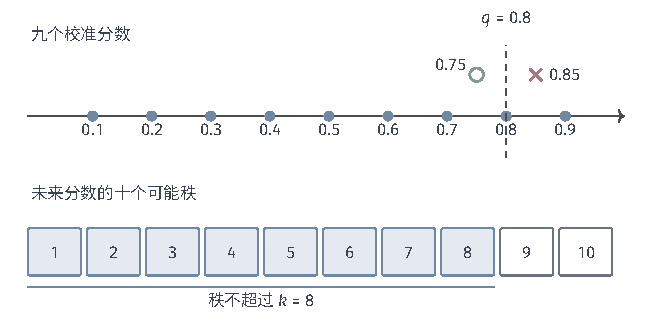
\includegraphics[width=111mm]{figures/00-shared/mathematical-preliminaries-lower/01-random-variables-distributions-and-causality/tikz/probability-conformal-ranks/source.pdf}
  \caption{拆分共形中的分数阈值与秩位置。上方取\(m=9\)、\(\alpha=0.2\)，校准值为\(0.1,\ldots,0.9\)，故\(k=8\)、\(q=0.8\)；空心圆候选分数\(0.75\)被纳入，叉号候选分数\(0.85\)被排除。下方浅色槽表示无并列可交换分数下未来秩不超过\(8\)的事件，其概率\(8/10\)针对校准与未来分数的联合抽样，而非给定上方校准值后的条件保证。}
  \label{fig:probability-conformal-ranks}
\end{figure}

\begin{theorem}[拆分共形的有限样本覆盖]
\label{thm:probability-split-conformal-coverage}
在上述条件下，
\[ \mathbb{P}\bigl(
    Y_{m+1}\in C(X_{m+1})\bigr)\geq 1-\alpha. \]
\end{theorem}

\begin{proof}
先假设分数无并列值。若未来真实标签未被覆盖，则\(S_{m+1}>q\)，所以未来分数在全部\(m+1\)个分数中的秩严格大于\(k\)。由式~\eqref{eq:probability-uniform-rank}，
\[ \mathbb{P}(S_{m+1}>q)
  =\mathbb{P}(R_{m+1}>k)=\frac{m+1-k}{m+1}\leq\alpha. \]
取补事件即得覆盖结论。

若有并列值，采用集合定义中的“\(\leq q\)”会把边界并列分数纳入预测集合。相较于随机打破并列后的精确秩，这只会增加覆盖事件，因此同一不等式仍成立。若希望得到更接近
精确的覆盖率，可显式随机化边界并列项，但必须把该随机化纳入算法与概率空间。
\end{proof}

这里的概率保证是\term{边际覆盖}：条件于训练数据后，它仍对随机的校准样本和未来样本共同取平均；若采用随机并列处理，还包括该随机性。解除对训练数据的条件后，总体覆盖率仍至少为
\(1-\alpha\)。但这个结论一般不推出对每个固定输入\(x\)都有
\[
  \mathbb{P}\bigl(
    Y_{m+1}\in C(X_{m+1})
    \mid X_{m+1}=x
  \bigr)
  \geq1-\alpha,
\]
也不自动保证每个群组内都达到同一覆盖率。逐输入、逐群组或时间条件覆盖需要额外结构、假设或专门的校准方法，不能仅由可交换秩推出。

证明依赖两处对称性。训练与校准拆分使评分规则在校准阶段保持固定；校准样本与未来样本可交换，使未来分数的秩没有特殊位置。若反复查看校准误差后修改模型或分数函数，评分规则
已依赖校准标签，条件可交换性可能被破坏。时间序列中的未来点通常也不能与过去点任意重排；自适应收集会让被选中的样本位置携带额外信息。此时失效的是均匀秩步骤，而不是把
分位数索引稍作调整就能修复。固定评分规则、校准与未来样本条件可交换时，本章的秩保证可以用于预测范围的边际覆盖；具体使用条件可参考
\BookChapterRef{chap:trust-reliability}{卷三的“可靠性”章}。
分组校准需要在看见校准结果前规定群组，并有足够的组内可交换样本。边际覆盖平均了输入位置，不自动给出每个连续输入处的条件覆盖。

\section{估计误差与效率}
\label{sec:stats-uncertainty-testing-selection}
一个估计数值需要评价平均损失或误差分布，一段参数范围需要评价重复抽样下的覆盖率，拒绝一个命题则需要控制误拒概率。评价标准由推断输出决定。重抽样、区间构造与检验程序都要在相应的抽样制度下建立保证；筛选数据或反复查看结果会改变该制度，因而必须重新核对条件。

\subsection{有限样本误差与线性估计效率}
\label{sec:statistics-bias-efficiency}
% Baseline T:446-459
估计量的误差既来自系统偏移，也来自样本波动。设标量估计量\(\widehat\theta\in L^2\)。对目标\(\theta\)，
\begin{align}
  \mathbb{E}[(\widehat\theta-\theta)^2]
  &=
  \mathbb{E}[(\widehat\theta-\mathbb{E}\widehat\theta
  +\mathbb{E}\widehat\theta-\theta)^2] \notag\\
  &=
  \operatorname{Var}(\widehat\theta)
  +\bigl(\mathbb{E}[\widehat\theta]-\theta\bigr)^2.
  \label{eq:statistics-mse-decomposition}
\end{align}
交叉项期望为零，因而均方误差等于方差加偏差平方。无偏不等于误差最小；少量偏差可能
换来更大的方差下降。

% Baseline T:470-498
若\(\bm\theta\in\mathbb{R}^d\)且\(\mathbb E\lVert\widehat{\bm\theta}\rVert_2^2<\infty\)，并使用总平方误差，则
\[
  \mathbb{E}\lVert\widehat{\bm\theta}-\bm\theta\rVert_2^2
  =\operatorname{tr}\{\operatorname{Cov}(\widehat{\bm\theta})\}
   +\lVert\mathbb{E}\widehat{\bm\theta}-\bm\theta\rVert_2^2.
\]
这不是每个坐标风险的最大值，也不是任意方向风险。

在高斯位置例子中，取固定中心\(\mu_0\)并令
\(\widetilde\theta=a\overline Y+(1-a)\mu_0\)，则
\[
  \operatorname{MSE}_\theta(\widetilde\theta)
  =\frac{a^2\sigma^2}{n}+(1-a)^2(\mu_0-\theta)^2.
\]
当\(\theta\)接近\(\mu_0\)时，某些\(a<1\)可比无偏的样本均值具有更小有限样本
均方误差；远离中心时，收缩偏差又可能占主导。比较结论必须固定目标、样本量和损失。

当任意\(\epsilon>0\)都满足
\(\mathbb{P}_\theta(|\widehat\theta_n-\theta|>\epsilon)\to0\)时，称估计量
\term{一致}（consistent）。一致性只描述样本量趋于无穷的极限，不给出当前样本的
误差，也不排除有限样本偏差。若
\(\mathbb{E}_\theta[(\widehat\theta_n-\theta)^2]\to0\)，则称为均方一致；
Markov不等式说明均方一致推出依概率一致，反向结论没有额外一致可积性时并不成立。
对某些满足额外正则条件的估计量，还能进一步证明
\[
  \sqrt n(\widehat\theta_n-\theta)
  \xrightarrow{\mathrm d}\mathcal N(0,V).
\]
这项性质称为渐近正态，它需要另行建立，并不由一致性自动推出。
% Baseline T:516-547
无偏性约束了平均位置，却尚未比较方差。把单一信号推广为一组带噪线性观测：给定设计矩阵\(\bm X\in\mathbb R^{n\times d}\)，设
\begin{equation}
  \bm Y=\bm X\bm\theta+\bm\varepsilon,\qquad
  \mathbb E[\bm\varepsilon\mid\bm X]=\bm0,\qquad
  \operatorname{Cov}(\bm\varepsilon\mid\bm X)=\sigma^2\bm I_n,
  \quad\sigma^2>0.
  \label{eq:statistics-gauss-markov-model}
\end{equation}
不同观测的条件噪声方差相同且协方差为零；这里不要求独立或高斯噪声。列满秩使参数可识别，最小二乘解为
\(\widehat{\bm\theta}=(\bm X^\top\bm X)^{-1}\bm X^\top\bm Y\)。它是否在所有无偏估计中最佳，需要先限定比较类。
\begin{theorem}[Gauss--Markov定理]
  \label{thm:statistics-gauss-markov}
  在式~\eqref{eq:statistics-gauss-markov-model}下，若\(\bm X\)列满秩，则\(\widehat{\bm\theta}\)条件无偏，且
  \(\operatorname{Cov}(\widehat{\bm\theta}\mid\bm X)=\sigma^2(\bm X^\top\bm X)^{-1}\)。
  对任何条件于\(\bm X\)固定、对全部\(\bm\theta\)均无偏的线性估计\(\widetilde{\bm\theta}=\bm C\bm Y\)，有
  \[
    \operatorname{Cov}(\widetilde{\bm\theta}\mid\bm X)
    -\operatorname{Cov}(\widehat{\bm\theta}\mid\bm X)\succeq\bm0.
  \]
\end{theorem}
\begin{proof}
记\(\bm C_0=(\bm X^\top\bm X)^{-1}\bm X^\top\)，于是\(\bm C_0\bm X=\bm I_d\)。直接对\(\bm C_0\bm Y\)求条件均值和协方差，得到无偏性及所述协方差。任一线性估计对所有参数无偏，等价于\(\bm C\bm X=\bm I_d\)。写\(\bm C=\bm C_0+\bm D\)，则\(\bm D\bm X=\bm0\)，从而
\[
  \bm C_0\bm D^\top
  =(\bm X^\top\bm X)^{-1}(\bm D\bm X)^\top=\bm0.
\]
展开\(\sigma^2\bm C\bm C^\top\)时两个交叉项都为零，故协方差之差为\(\sigma^2\bm D\bm D^\top\)。对任意向量\(\bm a\)，其二次型为\(\sigma^2\|\bm D^\top\bm a\|_2^2\geq0\)，即得半正定结论。
\end{proof}
半正定比较表示任意线性组合\(\bm a^\top\bm\theta\)的方差都不更大，强于只比较各坐标方差。定理的比较类是线性无偏估计，不排除前面那类有偏收缩估计获得更小均方误差，也不把异方差或相关噪声包含进来。

若\(\bm X=\bm1_n\)，参数就是共同均值，最小二乘退化为样本平均。任一无偏加权平均\(\sum_i a_iY_i\)满足\(\sum_i a_i=1\)；写\(a_i=1/n+b_i\)，则\(\sum_i b_i=0\)，其方差为
\(\sigma^2\sum_i a_i^2=\sigma^2/n+\sigma^2\sum_i b_i^2\)。额外的不均衡权重只增加方差，给出矩阵证明的一个可逐项核对的特例。
\subsection{渐近误差与估计方程的线性化}
% Baseline T:551-560
样本均值给出渐近正态的基本例子。若
\(Y_1,\ldots,Y_n\)独立同分布，且
\(\mathbb{E}[Y_i]=\theta\)、
\(0<\operatorname{Var}(Y_i)=\sigma^2<\infty\)，则中心极限定理给出
\[
  \sqrt n(\overline Y-\theta)
  \xrightarrow{\mathrm d}\mathcal N(0,\sigma^2).
\]
因此均值的渐近正态只需要有限方差，不要求观测本身服从高斯分布；在高斯位置模型中，
这个正态分布关系对每个有限\(n\)已经精确成立。
实际标准化常把未知方差换成样本估计。若样本方差一致，便可用\BookChapterRef{chap:random-sequences-and-processes}{第~\ref{chap:random-sequences-and-processes}章}的连续映射与Slutsky定理传递分布极限；这里只把这些运算用于估计误差，不重新建立一般收敛理论。

一般估计方程的渐近式还要控制在随机估计点附近的斜率。设\(Y_i\)独立同分布，且
\(\mathbb{E}[\psi(Y,\theta_0)]=0\)，记
\[
  A=\mathbb{E}[\partial_\theta\psi(Y,\theta_0)],
  \qquad B=\operatorname{Var}(\psi(Y,\theta_0)),
\]
要求\(A\neq0\)、\(B<\infty\)。一组足够条件是：\(\widehat\theta\)依概率趋于内点
\(\theta_0\)；\(\psi(y,\theta)\)在其某个邻域内连续可微；经验导数
\(n^{-1}\sum_i\partial_\theta\psi(Y_i,\theta)\)在该邻域上一致依概率收敛到
连续函数\(a(\theta)=\mathbb E[\partial_\theta\psi(Y,\theta)]\)；
估计方程残差\(r_n=n^{-1}\sum_i\psi(Y_i,\widehat\theta)\)满足
\(r_n=o_{\mathbb P}(n^{-1/2})\)。
一致性保证连接\(\theta_0\)与\(\widehat\theta\)的线段以趋于一的概率留在该邻域内。
沿线段积分导数，得到
\[
\begin{aligned}
 A_n&=\int_0^1\frac1n\sum_{i=1}^n
  \partial_\theta\psi\bigl(Y_i,\theta_0+t(\widehat\theta-\theta_0)\bigr)\,\mathrm dt
  \xrightarrow{\mathbb P}A,\\
 r_n&=\frac1n\sum_{i=1}^n\psi(Y_i,\theta_0)+A_n(\widehat\theta-\theta_0).
\end{aligned}
\]
随机斜率的收敛由一致导数控制与\(a\)的连续性共同给出，不能仅凭在固定点可微就断言。
因\(A\neq0\)，以趋于一的概率可以除以\(A_n\)；再由中心极限定理与Slutsky得到
\[
  \sqrt n(\widehat\theta-\theta_0)
  =
  -A^{-1}\frac1{\sqrt n}\sum_{i=1}^n\psi(Y_i,\theta_0)
  +o_{\mathbb{P}}(1),
\]
故极限方差为\(A^{-2}B\)，\(B=0\)时极限退化为零。多维情形将导数换为Jacobian，
要求其总体矩阵\(A\)非奇异，并对向量得分使用多元中心极限定理；极限协方差相应为
\(A^{-1}B(A^{-1})^\top\)，常称夹心协方差。模型正确的光滑似然在正则条件下可用
信息恒等式化简它；模型失配时\(A\)与\(B\)通常不再是同一个信息量，夹心两侧不能省略。

\subsection{Fisher信息与无偏估计的效率界}
均方误差评价一个给定估计量，效率界进一步询问同一观测模型允许的估计精度。
这里用对数似然的导数记录数据对参数的局部辨别能力；Fisher信息与统计几何章共用
同一个分布对象，定义见第~\ref{sec:information-fisher-geometry}节。本小节把得分用于无偏估计的误差下界。沿用标量得分\(u_\theta(y)=\partial_\theta\log p_\theta(y)\)，记\(\mathcal I(\theta)=\mathbb E_\theta u_\theta(Y_1)^2\)。独立样本的总得分为\(s_\theta(\bm Y)=\sum_{i=1}^n u_\theta(Y_i)\)；得分均值为零时，其方差为\(n\mathcal I(\theta)\)。

\begin{theorem}[Cramér--Rao下界]
\label{thm:statistics-cramer-rao}
设\(Y_1,\ldots,Y_n\)独立同分布于\(p_\theta\)，参数位于开区间，密度的支持不随参数改变，密度可对参数求导，归一化积分可交换求导与积分，得分的均值为零且方差等于Fisher信息。再设单样本
Fisher信息满足\(0<\mathcal I(\theta)<\infty\)。若\(\widehat\tau\)对可微目标
\(\tau(\theta)\)无偏、二阶矩有限，且其期望可对参数求导并移入积分，则
\[
  \operatorname{Var}_\theta(\widehat\tau)
  \geq\frac{\tau'(\theta)^2}{n\mathcal I(\theta)}.
\]
\end{theorem}

\begin{proof}
由无偏性\(\mathbb{E}_\theta[\widehat\tau]=\tau(\theta)\)对参数求导，并把导数移入积分，
得到
\[
  \tau'(\theta)
  =\mathbb{E}_\theta[
    (\widehat\tau-\tau(\theta))s_\theta(\bm Y)].
\]
Cauchy--Schwarz不等式给出
\[
  \tau'(\theta)^2\leq
  \operatorname{Var}_\theta(\widehat\tau)
  \operatorname{Var}_\theta(s_\theta(\bm Y))
  =
  \operatorname{Var}_\theta(\widehat\tau)n\mathcal I(\theta),
\]
整理即得结论。
\end{proof}

这个界不是所有估计问题的普遍极限。参数位于边界、支持依赖参数、模型不可识别或
Fisher信息奇异时，证明中的求导和除法可能失效；有偏估计量也要使用相应的偏差版本。
对\(\bm\theta\in\mathbb{R}^p\)和可微目标
\(\bm\tau(\bm\theta)\in\mathbb{R}^q\)，向量参数的正则版本为
\[
  \operatorname{Cov}_{\bm\theta}(\widehat{\bm\tau})
  \succeq
  \bm J_\tau(\bm\theta)\,
  \bm{\mathcal I}_n(\bm\theta)^{-1}\,
  \bm J_\tau(\bm\theta)^\top,
\]
其中\(\bm J_\tau\in\mathbb{R}^{q\times p}\)是目标映射的Jacobian，
\(\bm{\mathcal I}_n\)是整批样本的Fisher信息矩阵。这里要求信息矩阵可逆，
但Jacobian可以是矩形或降秩矩阵；估计参数本身时
\(\bm\tau(\bm\theta)=\bm\theta\)，故\(\bm J_\tau=\bm I_p\)。矩阵结论也不能由
逐坐标标量界直接拼接得到。
\section{区间估计与假设检验}
\label{sec:statistics-intervals-tests}
\subsection{区间估计的覆盖}
\subsubsection{固定样本下的覆盖与重抽样}
\label{sec:statistics-intervals-quantiles}
\label{sec:statistics-resampling}
% Baseline T:848-868
点估计没有说明误差尺度。覆盖区间需要先说明概率来自哪一次随机化，以及要覆盖的对象。
\begin{definition}[置信、可信与预测覆盖]
  \label{def:statistics-interval-coverage}
  取\(0<\alpha<1\)。\term{置信区间}（confidence interval）是一项重复抽样
程序：若每次按同一制度抽样并构造\(C(\bm Y)\)，则对模型中的每个\(\theta\)都有
\[
  \mathbb{P}_\theta\{\theta\in C(\bm Y)\}\geq1-\alpha.
\]
频率学派参数始终视作固定值；数据固定后，得到的区间也固定，不能把它解释为“以\(1-\alpha\)
概率包含参数”。Bayes\term{可信区间}（credible interval）则在给定数据和模型后
满足\(\mathbb{P}(\theta\in C\mid\bm y)\geq1-\alpha\)，其数值依赖先验；连续后验常可取到等号，离散后验可能只能给出更大的覆盖概率。
\term{预测集合}（prediction set）把覆盖对象改成未来结果，在规定的训练样本与未来
观测联合分布下要求
\(\mathbb{P}\{Y_{n+1}\in C(\bm Y)\}\geq1-\alpha\)。三者的概率分别来自重复样本、
参数后验，以及训练样本与未来观测的联合抽样，不能只按区间端点的外观解释。
\end{definition}

在独立同分布的高斯位置模型中，若方差已知，则
\[
  \frac{\overline Y-\theta}{\sigma/\sqrt n}\sim\mathcal N(0,1),
\]
% Baseline T:869-872
因而双侧置信区间为
\[
  \overline Y\pm z_{1-\alpha/2}\frac{\sigma}{\sqrt n}.
\]
这一区间覆盖固定均值，而第~\ref{sec:rv-prediction-sets}节的区间覆盖新观测。
取\(1-\alpha=0.95\)，对例~\ref{ex:statistics-running-sensor-calibration}，均值置信区间为
\[
10.4\pm1.96(2/5)=[9.62,11.18].
\]
它明显窄于下一次读数的预测区间\([6.40,14.40]\)，但不能替代后者。
% Baseline T:908-949

图~\ref{fig:statistics-mean-prediction-width}显示这一区分在样本量增长时仍然存在：均值标准误按\(n^{-1/2}\)减小，而未来单次读数的噪声不会因历史样本增多而消失。因此收集更多校准数据会把位置参数确定得更精确，却不能把一个有噪声的新读数限制到同样窄的范围。

\begin{figure}[!htb]
  \centering
  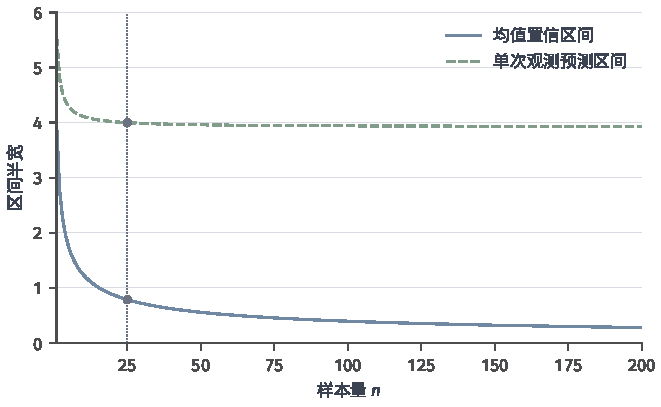
\includegraphics[width=\linewidth]{figures/00-shared/mathematical-preliminaries-lower/01-random-variables-distributions-and-causality/matplotlib/statistics-mean-prediction-width/figure.pdf}
  \caption{已知\(\sigma=2\)的独立高斯位置模型中，两类区间半宽随样本量变化（解析式教学图）。使用四舍五入分位数\(1.96\)，蓝实线为\(1.96\sigma/\sqrt n\)，绿虚线为\(1.96\sigma\sqrt{1+1/n}\)。灰竖线标出例~\ref{ex:statistics-running-sensor-calibration}的\(n=25\)，没有对任何实测数据重复抽样。}
  \label{fig:statistics-mean-prediction-width}
\end{figure}

\begin{table}[!htb]
  \centering
  \begin{tabular}{p{0.16\linewidth}p{0.29\linewidth}p{0.43\linewidth}}
    \toprule
    类型 & 覆盖对象 & 概率来源与必要条件\\
    \midrule
    置信区间 & 固定总体参数 & 同一抽样制度下重复构造区间的覆盖率\\
    可信区间 & 给定数据的参数后验 & 指定先验与似然形成的后验概率；不自动具有频率覆盖\\
    预测区间 & 尚未观测的随机结果 & 训练样本与未来观测的联合分布；须包含新观测波动\\
    \bottomrule
  \end{tabular}
  \caption{三类区间的覆盖对象与概率来源。区间形式相似时，仍须从所覆盖的对象解释结论。}
  \label{tab:statistics-interval-objects}
\end{table}

方差未知时，用
\[
  S^2=\frac1{n-1}\sum_{i=1}^n(Y_i-\overline Y)^2
\]
估计\(\sigma^2\)。在引理~\ref{lem:statistics-gaussian-mean-residual}的高斯独立样本条件下，
\[
  \frac{\overline Y-\theta}{S/\sqrt n}\sim t_{n-1},
\]
所以把高斯分位数换成\(t\)分位数可得到精确置信区间。这里的精确性依赖高斯性；
独立同分布、方差有限且为正的非高斯样本，配合样本方差的一致性，可由中心极限定理得到渐近近似；不满足这些条件的分布不能套用。样本很小且分布偏斜、重尾时，机械使用该区间可能同时
破坏中心和尾部覆盖。

双侧区间与双侧检验在相同模型、显著性水平和统计量下互为反演：若
\(\theta_0\)不在\(1-\alpha\)置信区间内，就拒绝\(H_0:\theta=\theta_0\)。
这种对应关系要求两者使用相同标准误与尾部规则。选择后区间、单侧检验或离散检验中，
不能只凭表面上的阈值照搬这一关系。
% Baseline T:1171-1228
复杂估计量的抽样分布难以解析计算时，可以用观测样本的经验分布模拟重复抽样。
\term{Bootstrap}从经验分布
\(\widehat P_n=n^{-1}\sum_i\Delta_{Y_i}\)有放回抽取\(n\)个观测，并重新计算
\(\widehat\tau^\ast\)。条件于原样本，\(\widehat\tau^\ast-\widehat\tau\)近似描述
\(\widehat\tau-\tau(P)\)的抽样波动。简单百分位区间取Bootstrap估计值的经验分位数，
但对不光滑统计量、边界参数、极端尾部分位数或重尾小样本，近似可能很差。

图~\ref{fig:statistics-bootstrap-layers}将这两层随机性分开：原抽样在固定总体\(P\)下产生随机观测\(\bm Y\)，Bootstrap计算则先固定已经获得的\(\bm Y\)，把每条观测记录赋权\(1/n\)，相同取值的权重合并，再从这个经验分布重新抽取。相应地，原误差以总体目标\(\tau(P)\)为中心，重抽样误差以当前估计\(\widehat\tau\)为中心。后者能否逼近前者的规律，需要下面的条件极限论证；重复重抽样只是更精细地计算给定经验分布下的波动，并不会增加来自总体的独立观测。

\begin{figure*}[htbp]
  \centering
  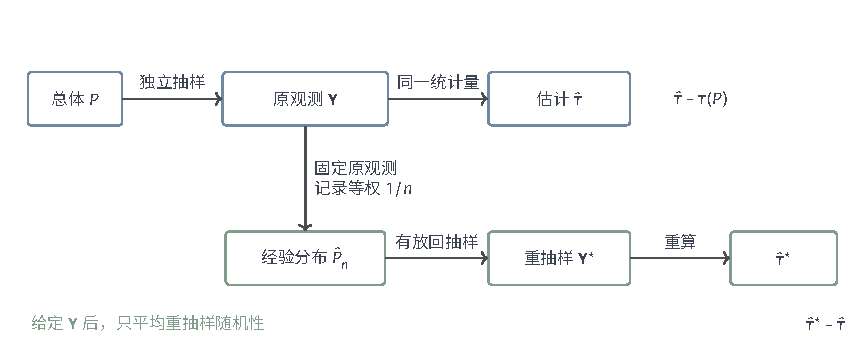
\includegraphics[width=145mm]{figures/00-shared/mathematical-preliminaries-lower/01-random-variables-distributions-and-causality/tikz/statistics-bootstrap-layers/source.pdf}
  \caption{原抽样与条件Bootstrap的两个随机层次。上行从总体\(P\)产生原观测并计算\(\widehat\tau\)，研究其相对\(\tau(P)\)的误差；下行固定同一批原观测，由经验分布\(\widehat P_n\)有放回抽取同样数量的观测，再用同一统计量重算\(\widehat\tau^\ast\)。下行的条件概率只平均重抽样随机性。两类中心化误差的分布能否相互逼近，仍需正文给出的有效性条件。}
  \label{fig:statistics-bootstrap-layers}
\end{figure*}

对独立同分布、方差\(0<\sigma^2<\infty\)的样本均值，这个近似有清楚的缩放口径。
若\(\overline Y^\ast\)由经验分布条件重抽样，则下述条件分布依概率弱收敛：
\[
  \mathcal L\!\left(
    \sqrt n(\overline Y^\ast-\overline Y)\mid\bm Y
  \right)
  \Longrightarrow\mathcal N(0,\sigma^2),
\]
与\(\sqrt n(\overline Y-\mu)\)的极限相同。这里条件分布随原样本而变，本身是随机对象。
具体地，用\(\mathbb E_\ast\)表示给定原数据后的重抽样期望，“依概率弱收敛”指
对每个有界Lipschitz函数\(f\)，
\[
 \mathbb E_\ast f\bigl(\sqrt n(\overline Y^\ast-\overline Y)\bigr)
 \xrightarrow{\mathbb P}\mathbb E f(Z),\qquad Z\sim\mathcal N(0,\sigma^2).
\]
外层的依概率收敛针对原数据的抽样随机性。

此处需要的中心极限定理允许抽样规律随\(n\)改变。
把随机变量逐行排列，第\(n\)行有\(n\)项\(X_{n,1},\ldots,X_{n,n}\)，
这样的排列称为三角阵列（triangular array）。
若每行内的变量独立、中心化，满足
\[
 \sum_{i=1}^n\mathbb E X_{n,i}^2\longrightarrow\sigma^2>0,\qquad
 \sum_{i=1}^n\mathbb E\!\left[
 X_{n,i}^2\mathbb I\{|X_{n,i}|>\varepsilon\}\right]\longrightarrow0
\]
对每个\(\varepsilon>0\)成立，则行和趋于\(\mathcal N(0,\sigma^2)\)。
第二项称为Lindeberg条件，排除了由少数单项主导总波动的情况。
这是所用的独立三角阵列中心极限定理；不要求不同行之间独立，完整证明见概率论教材\scite{math-kallenberg2021probability}。

对给定原数据的重抽样取\(X_{n,i}=(Y_i^\ast-\overline Y)/\sqrt n\)。
行和就是所研究的均值波动；条件均值为零，条件方差和是经验方差。
经验均值等于\(\overline Y\)，经验方差
依概率趋于\(\sigma^2\)，但方差收敛本身还不足以保证条件中心极限定理。有限二阶矩还使
每个\(\varepsilon>0\)对应的条件Lindeberg尾项满足
\[
  \frac1n\sum_{i=1}^n(Y_i-\overline Y)^2
  \mathbb I\{|Y_i-\overline Y|>\varepsilon\sqrt n\}
  \xrightarrow{\mathbb P}0.
\]
这个经验尾项恰好是上述阵列在条件分布下的Lindeberg和。
其收敛可直接由有限二阶矩核对。以趋于一的概率
\(|\overline Y-\mu|\leq\varepsilon\sqrt n/2\)；在此事件上，
若\(|Y_i-\overline Y|>\varepsilon\sqrt n\)，则
\(|Y_i-\mu|>\varepsilon\sqrt n/2\)。又有
\[
 (Y_i-\overline Y)^2\leq2(Y_i-\mu)^2+2(\overline Y-\mu)^2.
\]
因此经验尾项被原中心平方尾的两倍经验平均加\(2(\overline Y-\mu)^2\)控制。
第一项的期望随截断阈值增大而趋零，由Markov不等式依概率趋零；第二项由大数定律趋零。

为把随机条件量接到确定阵列定理，可从任意原数据子列中再抽出一条子子列，
使经验方差和所有正有理\(\varepsilon\)的尾项同时几乎必然收敛；
这是\BookLemmaRef{lem:rv-probability-subsequence}{引理~\ref{lem:rv-probability-subsequence}}的可数对角应用。
尾项关于阈值单调，故该共同满测集上所有正阈值的条件都成立。
逐条固定这样的原数据实现，应用阵列定理便得到条件弱收敛；
再用同一子列判据返回上述测试函数积分的依概率结论。
该结论针对中心化、缩放后的条件分布；它本身不自动证明任意百分位
区间具有高阶准确性。

例~\ref{ex:statistics-running-sensor-calibration}中的经验分布均值为\(10.4\)，经验
方差按分母\(n\)计算恰为\(4\)。因此单次Bootstrap抽样值满足
\[
  \mathbb{E}_\ast[Y^\ast]=10.4,\qquad
  \operatorname{Var}_\ast(Y^\ast)=4,
\]
而二十五次有放回抽样的均值满足
\[
  \operatorname{SE}_\ast(\overline Y^\ast)
  =
  \sqrt{\frac4{25}}=0.4.
\]
若中心化并按标准误标准化后的条件Bootstrap分布可由标准正态分布近似，则正态
Bootstrap区间为
\(10.4\pm1.96\times0.4=[9.62,11.18]\)，与已知方差高斯区间在这个构造例中重合。
重合来自经验方差刚好等于已知噪声方差以及均值的光滑性，不是Bootstrap总会复制参数
区间的保证。

更一般的统计量可以用线性化研究，但须分别控制原抽样与重抽样的余项。即使已经证明
\[
  \widehat\tau-\tau(P)
  =
  \frac1n\sum_{i=1}^n\operatorname{IF}(Y_i;T,P)
  +o_{\mathbb{P}}(n^{-1/2}),
\]
也还需证明条件重抽样展开，例如对某个数据依赖的中心化函数\(\phi_n\)，
\[
 \widehat\tau^\ast-\widehat\tau
 =\frac1n\sum_{i=1}^n\phi_n(Y_i^\ast)+r_n^\ast,\qquad
 \mathbb E_\ast\phi_n(Y_i^\ast)=0.
\]
所需余项条件是：对每个\(\varepsilon>0\)，
\(\mathbb P_\ast(\sqrt n|r_n^\ast|>\varepsilon)\xrightarrow{\mathbb P}0\)；
这就是这里的条件\(o_{\mathbb P_\ast}(n^{-1/2})\)。
若经验影响函数\(\phi_n\)还满足条件中心极限定理，且极限方差与原影响函数一致，
两边缩放后的分布才趋于同一极限。适当的统计泛函光滑性可以帮助建立这些条件，
不能只把原展开中的\(P\)换成\(\widehat P_n\)便认定已证明Bootstrap有效\scite{vanderVaart1998asymptotic}。

一个短反例说明为何必须单独检查重抽样。连续有限方差分布下，取
\[
 \widehat\tau_n=\overline Y+n^{-1/2}
 \mathbb I\{\text{样本中有重复值}\}.
\]
原样本几乎必然没有重复值，所以它具有与均值完全相同的原抽样展开。
但从\(n\)个不同观测有放回抽\(n\)次，全不重复的条件概率为
\(n!/n^n\leq\exp(-(n-1)/2)\)，趋于零；不等式来自
\(\log(1-j/n)\leq-j/n\)的逐项求和。
于是\(\sqrt n(\widehat\tau_n^\ast-\widehat\tau_n)\)额外平移约\(1\)，
没有逼近原统计量的中心化极限。
样本最大值之类统计量
没有这种常规线性展开：经验分布不会生成比当前最大值更大的观测，简单Bootstrap便可能
错误描述尾部。
% Baseline T:1247-1249
重采样单位必须跟独立单位一致。配对实验对整对数据重采样；多个记录属于同一用户时对
用户群组重采样；时间相关数据使用保留局部依赖的块Bootstrap。逐条重采样会把共享噪声
误当作独立波动，通常低估标准误。
\subsubsection{序贯覆盖与可预测设计}
% Baseline S:642-649
重采样解决的是固定程序的误差近似；不断增加样本并反复查看区间，还增加了停止规则的问题。若每次查看都各自给出同一覆盖率，不能推出全部查看同时覆盖。需要把保证改成一个共同事件：真实参数在所有时刻的区间内，这样根据已有数据停止时仍可继承覆盖。
\begin{definition}[置信序列]
  \label{def:stoch-confidence-sequence}
  对参数为\(\theta\)时的数据分布\(\mathbb P_\theta\)，数据依赖集合\((C_t)_{t\geq1}\)若在时刻\(t\)由\(\mathcal F_t\)确定，且对每个允许的\(\theta\)满足
  \[ \mathbb P_\theta(\theta\in C_t\text{ 对所有 }t\geq1)\geq1-\delta, \]
  则称为覆盖水平\(1-\delta\)的\term{置信序列}（confidence sequence），其中\(0<\delta<1\)。
\end{definition}
它在同一个高概率事件上覆盖所有时刻，因而允许根据当前数据决定何时查看或停止。固定$n$的置信区间只承诺
预先指定时刻的覆盖；反复查看直到区间排除某个值，会改变错误概率。
一个可直接计算的标量构造来自Hoeffding界。若\(X_i\in[0,1]\)独立同分布，均值为
\(\mu\)，给第\(n\)次查看分配错误预算
\(\delta_n=\delta/[n(n+1)]\)，则\(\sum_{n\geq1}\delta_n=\delta\)。定义
\[
C_n=\left[\overline X_n-
\sqrt{\frac{\log(2n(n+1)/\delta)}{2n}},
\ \overline X_n+
\sqrt{\frac{\log(2n(n+1)/\delta)}{2n}}\right]\cap[0,1].
\]
对全部时刻的坏事件取并集，即得
\(\mathbb P(\forall n,\mu\in C_n)\geq1-\delta\)。
取\(\delta=0.05,n=100\)，半宽约为\(0.254\)；固定时刻Hoeffding区间半宽约为
\(0.136\)。同时保证付出了更宽范围，这个简单预算构造也不是最紧的边界。条件均值恒为
\(\mu\)且条件范围仍为\([0,1]\)时，条件Hoeffding论证给出同样控制；任意相关观测则不能直接使用。
预先固定有限个候选时，可再将\(\delta\)分给各候选以保证选择后的覆盖。无限搜索或用同一数据重新设计目标，需要额外统一控制或独立评价数据。

对于可预测的向量设计，下面回用\BookSectionRef{sec:rv-anytime}{第~\ref{sec:rv-anytime}节}的自归一化界，把累计噪声转成参数置信椭球。
% Baseline S:816-924
取$\bm{V}_0=\lambda\bm{I}$，$\lambda>0$，并定义岭回归估计
\begin{equation}
  \widehat{\bm{\theta}}_t
  =\bm{V}_t^{-1}\sum_{s=1}^{t}\bm{x}_s y_s.
  \label{eq:stoch-ridge-estimator}
\end{equation}
由\BookEquationRef{eq:stoch-adaptive-linear-observation}{式~\eqref{eq:stoch-adaptive-linear-observation}}，
\[
  \bm{V}_t
  (\widehat{\bm{\theta}}_t-\bm{\theta}^{\star})
  =
  \bm{S}_t-\lambda\bm{\theta}^{\star}.
  \]
若还知道$\lVert\bm{\theta}^{\star}\rVert_2\leq B$，三角不等式给出
\begin{align}
  \lVert
    \widehat{\bm{\theta}}_t-\bm{\theta}^{\star}
  \rVert_{\bm{V}_t}
  &\leq
  \lVert\bm{S}_t\rVert_{\bm{V}_t^{-1}}
  +
  \lambda
  \lVert\bm{\theta}^{\star}\rVert_{\bm{V}_t^{-1}}
  \notag\\
  &\leq
  R\sqrt{
    2\log\left(
      \frac{\det(\bm{V}_t)^{1/2}}
           {\lambda^{d/2}\delta}
    \right)
  }
  +\sqrt{\lambda}B
  =:\beta_t(\delta).
  \label{eq:stoch-adaptive-confidence-ellipsoid}
\end{align}
第二个不等式使用$\bm{V}_t\succeq\lambda\bm{I}$。因此
\[
  \mathcal{C}_t(\delta)
  =
  \left\{
    \bm{\theta}:
    \lVert\bm{\theta}-\widehat{\bm{\theta}}_t
    \rVert_{\bm{V}_t}
    \leq\beta_t(\delta)
  \right\}
\]
在同一个概率至少为$1-\delta$的事件上，对所有$t$都包含真实参数。这是置信椭球而不是
欧氏球：观测充分的方向较窄，信息不足的方向较宽。

\begin{example}[二维自适应查询]
  \label{ex:stoch-two-dimensional-adaptive-design}
  设$d=2$、$\lambda=1$，每次只能在
  $\bm{e}_1=(1,0)^\top$与$\bm{e}_2=(0,1)^\top$中选择一个观测方向。算法在第
  $t$步根据上一轮椭球在两个方向上的宽度调整查询概率，再抽取方向：所用随机数在给定此前历史后服从\(\operatorname{Unif}(0,1)\)，并与当前噪声条件独立，且在噪声出现前完成抽取。较宽的方向获得较大概率，但不必每次选中；把这次抽取纳入观测前的信息后，$\bm{x}_t$可预测，噪声的条件次高斯界也保持。

  若前四次选择中$\bm{e}_1$出现三次、$\bm{e}_2$出现一次，则
  \[
    \bm{V}_4
    =
    \begin{pmatrix}
      4&0\\
      0&2
    \end{pmatrix},
    \qquad
    \det(\bm{V}_4)=8.
  \]
  对任意方向$\bm{x}$，椭球给出的预测误差满足
  \[
    |\langle
      \bm{x},
      \widehat{\bm{\theta}}_4-\bm{\theta}^{\star}
    \rangle|
    \leq
    \beta_4(\delta)
    \lVert\bm{x}\rVert_{\bm{V}_4^{-1}}.
  \]
  因而两个坐标方向的半宽分别与$1/2$和$1/\sqrt2$成比例。第一个方向访问更多，区间
  更窄；下一次提高第二个方向的查询概率，是由已有信息决定的自适应设计。定理仍然适用，因为它在每次
  新噪声产生之前固定当前方向，并在一个事件上同时控制全部时刻。
\end{example}

图~\ref{fig:stochastic-design-ellipsoids}还比较了相同四次预算在两个方向各访问两次的情形：此时\(\bm V_4=\operatorname{diag}(3,3)\)。均衡访问扩大第一个方向的几何半宽，却缩小第二个方向的半宽；因此设计会改变误差的方向分配，不能只比较一个总访问数。图中把两条二次型的右侧统一设为\(1\)，仅比较几何；真正的置信椭球还要分别乘上各自的\(\beta_4(\delta)\)，其行列式项也会改变。

\begin{figure}[htbp]
  \centering
  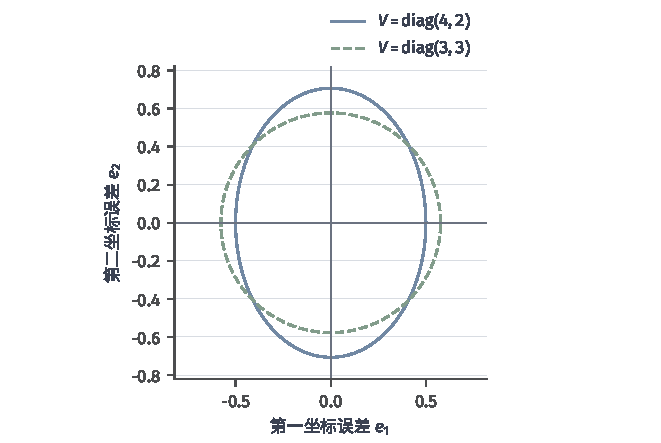
\includegraphics[width=\linewidth]{figures/00-shared/mathematical-preliminaries-lower/01-random-variables-distributions-and-causality/matplotlib/stochastic-design-ellipsoids/figure.pdf}
  \caption{二维设计的归一化误差几何（解析式教学图）。蓝实线为\(\bm e^\top\operatorname{diag}(4,2)\bm e=1\)，绿虚线为\(\bm e^\top\operatorname{diag}(3,3)\bm e=1\)。它们不是已经具有相同覆盖概率的数值置信区间；真实置信半径由式~\eqref{eq:stoch-adaptive-confidence-ellipsoid}另行确定。}
  \label{fig:stochastic-design-ellipsoids}
\end{figure}

这个例子也说明为什么不能把独立样本界中的$n$换成某个动作的访问次数。参数误差是向量，
不同特征方向可能相关；置信宽度由$\bm{x}^{\top}\bm{V}_t^{-1}\bm{x}$决定，而不是只由
某个坐标被访问多少次决定。行列式项又要为算法可能探索的全部方向支付复杂度。

\paragraph{可预测设计与数据依赖的边界}
自归一化界允许$\bm{x}_t$依赖$\mathcal{F}_{t-1}$，不允许它依赖当前$\eta_t$后再伪装成
预先选择。若传感器先看到当前噪声再决定是否记录，$\bm{x}_t\eta_t$的条件平均可能不再为
零，指数超鞅的第一步就会失败。类似地，模型失配使
$\mathbb{E}[y_t\mid\mathcal{F}_{t-1},\bm{x}_t]$不等于
$\langle\bm{x}_t,\bm{\theta}^{\star}\rangle$时，估计误差中会增加系统偏差，原半径没有证明能控制这项偏差，
不能继续给出同一个真实参数的原覆盖保证。

条件次高斯性也不是有限方差的同义词。重尾噪声可能需要截断、稳健均值或只使用有限矩的
其他序贯工具；直接套用\BookEquationRef{eq:stoch-vector-self-normalized-bound}{式~\eqref{eq:stoch-vector-self-normalized-bound}}会低估尾部。
$\lambda$保证初期矩阵可逆并编码参数范数先验，但过大的$\lambda$会增加
$\sqrt{\lambda}B$偏差项。置信椭球控制统计误差，不保证选择策略会访问所有对任务重要的
方向；探索是否充分仍要由设计规则与任务目标另行证明。

\subsection{假设检验的错误控制}
\subsubsection{检验目标、证据与功效}
\label{sec:statistics-testing-errors}
\label{sec:statistics-selection-multiplicity}
% Baseline T:1012-1164
区间描述目标的可能范围，\term{假设检验}（hypothesis testing）则检查数据与一个
命题是否相容。
一个确定性规则对每组记录只作拒绝或不拒绝两种选择。但在离散观测中，直接增加一整个拒绝事件可能使误拒概率超过预算；允许在边界记录上再随机拒绝，可以细调这项概率。于是用取值于\([0,1]\)的函数统一表示拒绝概率，确定性规则对应只取\(0,1\)的特例。
\begin{definition}[随机化检验函数]
  \label{def:statistics-randomized-test-function}
  若单个观测的可测空间为\(\mathcal{Y}\)，则
  \term{随机化检验函数}（randomized test function）是可测映射
  \[
    \varphi:\mathcal{Y}^n\to[0,1].
  \]
  观察到\(\bm{Y}=\bm{y}\)后，检验以概率\(\varphi(\bm{y})\)拒绝原假设。等价地，可另取
  独立的\(U\sim\operatorname{Unif}(0,1)\)，并在
  \(U\leq\varphi(\bm{y})\)时拒绝。只取\(0,1\)值的检验是非随机化特例，其拒绝域为
  \(R=\{\bm{y}:\varphi(\bm{y})=1\}\)。
\end{definition}

原假设\(H_0\)指定被控制误报的情形。检验的大小与参数\(\theta\)下的功效分别为
\[
  \sup_{\theta\in H_0}\mathbb{E}_\theta[\varphi(\bm Y)],
  \qquad
  \mathbb{E}_\theta[\varphi(\bm Y)].
\]
水平为\(\alpha\)要求
\[
  \sup_{\theta\in H_0}
  \mathbb{E}_\theta[\varphi(\bm Y)]
  \leq\alpha.
\]
在\(H_0\)为真时拒绝是第一类错误；在备择\(H_1\)为真时不拒绝是第二类错误。
对非随机化检验，这些期望分别退化为拒绝域概率。效应量描述差异有多大，样本量则影响
能否把该差异从噪声中区分出来。

\term{\(p\)值}（\(p\)-value）的一种常见构造，是在原假设下计算至少与当前统计量同样极端结果的概率。复合假设或其他构造还需满足下面的有效性要求。
\begin{definition}[有效p值]
  \label{def:statistics-valid-p-value}
  一个取值于\([0,1]\)的可测统计量\(p(\bm Y)\)是复合原假设\(H_0\)下的有效\(p\)值，若对每个
\(u\in[0,1]\)都有
\[
  \sup_{\theta\in H_0}\mathbb{P}_\theta\{p(\bm Y)\leq u\}\leq u.
\]
\end{definition}
这项零假设下的超均匀性质才保证按阈值\(\alpha\)拒绝时控制第一类错误。观察到的
\(p\)值不是原假设为真的概率，也不是效应量。仍取已知\(\sigma\)的高斯位置模型，
检验\(H_0:\theta=0\)时
\[
  Z=\frac{\sqrt n\,\overline Y}{\sigma},\qquad
  p=2\{1-\Phi(|Z|)\}.
\]
若\(\theta=\delta\)，双侧检验功效为
\[
  \mathbb{P}_\delta(|Z|>z_{1-\alpha/2})
  =
  1-\Phi\left(z_{1-\alpha/2}-\frac{\sqrt n\delta}{\sigma}\right)
  +\Phi\left(-z_{1-\alpha/2}-\frac{\sqrt n\delta}{\sigma}\right).
\]
小样本下“不显著”可能只表示功效不足。保持观测到的\(|\overline Y|>0\)及\(\sigma>0\)不变时，增大\(n\)会使上式的\(p\)值变小；固定真实效应的另一次抽样却不保证\(p\)值逐次减小。

检验族还可反演为置信集合。对每个候选值\(\theta_0\)，设
\(\varphi_{\theta_0}(\bm Y)\in\{0,1\}\)是水平不超过\(\alpha\)的检验，并定义
\[
  C(\bm Y)=\{\theta_0:\varphi_{\theta_0}(\bm Y)=0\}.
\]
当真实值为\(\theta\)时，
\[
  \mathbb{P}_\theta\{\theta\notin C(\bm Y)\}
  =\mathbb{P}_\theta\{\varphi_\theta(\bm Y)=1\}\leq\alpha,
\]
所以\(C\)具有至少\(1-\alpha\)覆盖率。这里必须对同一模型、同一尾部规则和同一
标准误反演；选择后换检验或只挑有利方向会破坏证明。

\begin{example}[同一效应量下的证据与功效]
\label{ex:statistics-evidence-power-same-effect}
设噪声标准差已知为\(\sigma=2\)，观测均值为\(\overline y=1\)，检验
\(H_0:\theta=0\)。当\(n=4\)时，\(Z=1\)，双侧\(p\)值约为\(0.317\)；
当\(n=100\)时，\(Z=5\)，双侧\(p\)值小于\(10^{-6}\)。两次实验报告的标准化
效应\(\overline y/\sigma=0.5\)相同，证据强度却因标准误不同而变化。

若真实值确为\(\delta=1\)，显著性水平为\(0.05\)，则\(n=4\)时双侧检验功效约为
\[
  1-\Phi(1.96-1)+\Phi(-1.96-1)\approx0.17.
\]
此时未拒绝原假设并不支持“差异为零”。若实际问题把绝对差异不超过\(0.2\)视为等效，
还需要针对\(\Delta=0.2\)设计等效检验；当前样本对这个更严格目标几乎没有辨识力。
\end{example}

\paragraph{似然比排序与Neyman–Pearson引理}
固定允许的误拒概率后，希望尽量提高识别另一个指定规律的概率。对同一份记录，若它在备择规律下比在原假设下更常见，就应优先把它放入拒绝域；似然比给出这个相对证据的排序，阈值再用完允许的错误预算。
下面的经典引理给出两个简单假设之间的最强检验\scite{math-lehmann2005testing}。
\begin{theorem}[Neyman--Pearson引理]
\label{thm:statistics-neyman-pearson}
取\(0<\alpha<1\)。对两个完全指定的简单假设\(H_0:P=P_0\)与\(H_1:P=P_1\)，设
\(P_1\ll P_0\)，似然比为\(\Lambda=\mathrm dP_1/\mathrm dP_0\)。在所有大小
不超过\(\alpha\)的检验中，拒绝大似然比并在边界适当随机化的检验具有最大功效。
\end{theorem}

\begin{proof}
取常数\(c\geq0\)与边界随机化概率，使检验\(\varphi^\star\)满足
\(\mathbb{E}_0[\varphi^\star]=\alpha\)，并在\(\Lambda>c\)时拒绝、在
\(\Lambda<c\)时接受。对任意\(\mathbb{E}_0[\varphi]\leq\alpha\)的检验，
\[
  (\varphi^\star-\varphi)(\Lambda-c)\geq0
\]
逐点成立，因为\(\varphi^\star\)在\(\Lambda>c\)处取最大允许值，在
\(\Lambda<c\)处取最小允许值。对\(P_0\)积分得到
\[
  \mathbb{E}_1[\varphi^\star-\varphi]
  \geq c\,\mathbb{E}_0[\varphi^\star-\varphi]\geq0.
\]
所以\(\varphi^\star\)的备择拒绝概率不小于任何同大小检验。
\end{proof}

这个结论只直接覆盖两个简单假设。复合假设需要处理未知参数，不一定存在一致最强检验。
在隐私攻击审计中，\(P_0\)与\(P_1\)可分别表示目标记录不在与在训练集时的输出分布；
似然比给出理想攻击排序，但实际审计还要估计这两个分布并计入选择偏差。

\subsubsection{分类观测与随机化检验}
两个分类变量的列联表中，原假设为独立时，期望格数是
\[
  E_{r,c}=\frac{N_{r,\cdot}N_{\cdot,c}}{N},\qquad
  X^2=\sum_{r,c}\frac{(N_{r,c}-E_{r,c})^2}{E_{r,c}}.
\]
计算时先删去零边际计数的行列，保证保留格子的\(E_{r,c}>0\)。当样本独立同分布、类别数\(R,C\)固定，且原假设下各格子的总体概率为正时，随\(N\to\infty\)，
\(X^2\)的分布趋于自由度\((R-1)(C-1)\)的卡方分布。稀疏格数会破坏近似，可合并有
科学意义的类别或使用精确、置换方法。条件独立检验还要控制第三个变量；把样本简单切成
大量小层会带来新的稀疏性，不能由普通卡方检验自动解决。

差异检验把“无差异”放在原假设中。等效性检验先给出有实际含义的可接受差异界
\(\Delta>0\)。记\(\delta=\theta_A-\theta_B\)，两个单侧检验（two one-sided
tests, TOST）把不等效原假设写成两个集合的并：
\[
  H_0=H_{0,L}\cup H_{0,U},
  \qquad
  H_{0,L}:\delta\leq-\Delta,
  \qquad
  H_{0,U}:\delta\geq\Delta.
\]
对应备择为\(-\Delta<\delta<\Delta\)。TOST只有在水平\(\alpha\)的下侧检验拒绝
\(H_{0,L}\)，并且水平\(\alpha\)的上侧检验也拒绝\(H_{0,U}\)时，才拒绝总体原假设。
取\(0<\alpha<1/2\)。例如，若\(\widehat\delta\)的标准误为\(s>0\)，且标准化统计量服从相应正态近似，
拒绝条件为
\begin{equation}
  \frac{\widehat\delta+\Delta}{s}>z_{1-\alpha}
  \quad\text{且}\quad
  \frac{\widehat\delta-\Delta}{s}<z_{\alpha}.
  \label{eq:statistics-tost-rejection}
\end{equation}
这等价于把双侧\(1-2\alpha\)置信区间完整放入
\((-\Delta,\Delta)\)。总体第一类错误并非\(2\alpha\)：只要
\(\delta\in H_0\)，至少有一个单侧原假设为真，而总体拒绝事件包含在拒绝这个真原假设
的事件中，所以其概率至多为\(\alpha\)。非劣效检验只排除一个方向，例如
\(H_0:\delta\leq-\Delta\)。未拒绝差异检验的零假设不等于证明等效。
图~\ref{fig:statistics-difference-equivalence}把这两个判据放在同一个差异轴上。蓝色区间检查零点是否被排除，绿色区间检查它是否完整位于预先规定的等效界内。第一行的区间太宽，既不能排除零，也不能排除具有实际意义的差异；第二行围绕零且足够窄，可以支持等效。第三行的差异虽已足以排除零，其范围仍完整位于等效界内，因此“统计上非零”与“在指定尺度下等效”可以同时成立。两个检验回答的问题不同，不能仅用是否显著替代实际差异范围的判断。

\begin{figure}[htbp]
  \centering
  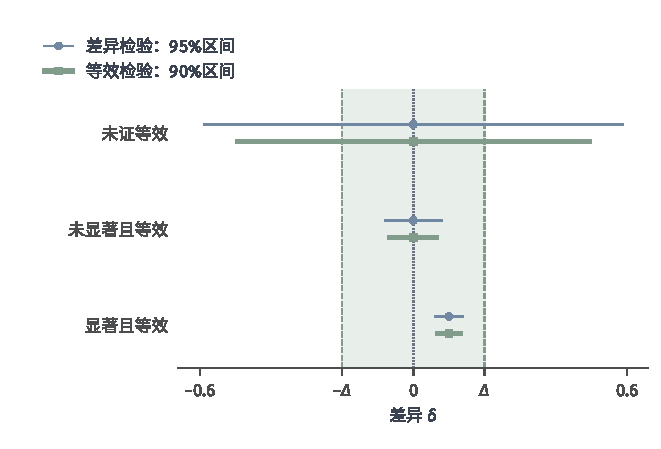
\includegraphics[width=112mm]{figures/00-shared/mathematical-preliminaries-lower/01-random-variables-distributions-and-causality/matplotlib/statistics-difference-equivalence/figure.pdf}
  \caption{差异检验与等效检验的区间判读。教学设定为已知标准误的正态差异估计，\(\alpha=0.05\)、\(\Delta=0.2\)；三行\((\widehat\delta,s)\)依次为\((0,0.30)\)、\((0,0.04)\)、\((0.10,0.02)\)。蓝细线为差异检验对应的\(95\%\)区间，绿粗线为TOST对应的\(90\%\)区间，浅绿带表示\((-\Delta,\Delta)\)。第三行同时排除零并支持等效；两类区间使用不同覆盖水平，不能互换。}
  \label{fig:statistics-difference-equivalence}
\end{figure}

% Baseline T:1232-1245
\term{置换检验}（permutation test）近似的不是估计量抽样分布，而是零假设下标签可
交换时的随机化分布。两组观测在“处理标签不影响联合分布”的原假设下，可反复打乱标签
并重算组间差异。若分配机制只允许在区组内交换，就必须在区组内置换；任意全局打乱会
制造实验中不可能出现的分配。

设允许的置换构成一个含\(M\)个元素的有限群，原假设下观测联合分布在该群作用下不变。把观测统计量与全部群置换统计量一起排序；没有并列时，群对称性使秩具有均匀规律，存在并列时使用
\[
  p_{\mathrm{perm}}
  =\frac{\#\{\text{置换统计量不小于观测值}\}}{M}
\]
得到超均匀而可能保守的\(p\)值。若独立、均匀地从该群抽取\(B\)个置换，常用
\((1+\#\{\text{抽样置换不小于观测值}\})/(B+1)\)保留有限模拟下的保守性。
仅有两组均值相等并不保证整批标签可交换；交换性必须来自更强的零假设或随机分配设计。
\subsubsection{多重比较与序贯查看的错误控制}
% Baseline T:1256-1293
单个检验的第一类错误为\(\alpha\)，不代表同时尝试许多候选后仍只有
\(\alpha\)的误报概率。若\(m\)个原假设都为真，联合界给出
\[
  \mathbb{P}(\text{至少一次误拒绝})
  \leq\sum_{j=1}^m\mathbb{P}(\text{拒绝 }H_j)
  \leq m\alpha.
\]
Bonferroni方法把每项阈值设为\(\alpha/m\)，从而控制
\term{族错误率}（family-wise error rate, FWER）。它不要求检验独立，但候选很多时
可能保守。

Holm方法把\(p\)值从小到大排序，并依次将
\(p_{(j)}\)与\(\alpha/(m-j+1)\)比较，遇到第一个未拒绝项即停止。若第一个被错误
拒绝的真原假设位于位置\(j\)，设真原假设总数为\(m_0\)，则前\(j-1\)项均为假
原假设，所以\(m-j+1\geq m_0\)。该真原假设的\(p\)值因而不超过
\(\alpha/(m-j+1)\leq\alpha/m_0\)。对全部\(m_0\)个真原假设应用联合界，便把
发生任一错误拒绝的概率控制在\(\alpha\)以内。它与Bonferroni一样不要求独立，但利用
了逐步比较。

当目标是控制所有拒绝中错误发现的期望比例时，可使用
\term{错误发现率}（false discovery rate, FDR）。设\(R\)为拒绝的总数、\(V\)为其中
被错误拒绝的真原假设数，则
\[
  \operatorname{FDR}=\mathbb E\left[\frac{V}{\max(R,1)}\right].
\]
当\(R=0\)时，错误发现比例约定为零；这是随机比例的期望，不是
\(\mathbb EV/\mathbb ER\)。Benjamini--Hochberg过程将
\(p\)值排序为\(p_{(1)}\leq\cdots\leq p_{(m)}\)，找最大
\[
  k=\max\left\{j:p_{(j)}\leq\frac{j}{m}q\right\},
\]
并拒绝前\(k\)项；若集合为空，则取\(k=0\)，不拒绝任何假设。若全部\(p\)值相互
独立，且每个真原假设下的\(p\)值满足
\(\mathbb P(p_j\leq u)\leq u\)（\(0\leq u\leq1\)），该过程控制FDR不超过目标
\(q\in(0,1)\)\scite{statistics-benjamini-hochberg1995}。扩展到依赖检验需要更精确的联合分布条件，不能仅凭两两正相关或任意
依赖就沿用这项保证。

从多个模型中挑选测试误差最小者，再把该最小值当成固定模型的无偏评估，通常会引入选择后的乐观偏差。
% Baseline T:1330-1343
持续查看同一数据也构成选择。固定时刻满足
\(\mathbb{P}(p_t\leq\alpha)\leq\alpha\)并不推出
\(\mathbb{P}(\exists t:p_t\leq\alpha)\leq\alpha\)。预先规定查看次数可分配
\(\alpha\)预算；更灵活的停止规则需要序贯检验、置信序列或对整个证据过程的控制。
停止规则属于推断程序的一部分，不能在看到结果后删去。

一种单次证据是\(e\)值（e-value）：非负统计量\(E\)若在每个零假设分布\(P\)下
满足\(\mathbb E_PE\leq1\)，就称为有效\(e\)值。由Markov不等式，
\(P(E\geq1/\alpha)\leq\alpha\)，所以大值可以用来拒绝零假设。
但逐个固定时刻的\(E_t\)都是有效\(e\)值，仍不足以保证可以任意停止；
下文用非负超鞅给出一种能同时控制所有时刻的证据过程。

定义~\ref{def:stoch-confidence-sequence}的\term{置信序列}（confidence sequence）把所有时刻的覆盖放在同一个高概率事件中。这比每个固定时刻各自覆盖更强，因为允许依据当前数据决定何时停止查看。
若\((E_t)\)在原假设下是从\(E_0=1\)开始的非负超鞅，则Ville不等式给出
\[
  \mathbb{P}_0\left\{\sup_{t\geq0}E_t\geq\frac1\alpha\right\}\leq\alpha.
\]
因此可以在任意由过去信息决定的停止时刻按阈值查看\(E_t\)，而不增加这项越界概率。
这不表示停止后的点估计无偏，也不表示同时尝试多个证据过程无需额外控制；覆盖、估计
偏差和模型选择证据仍是不同问题。

\section{有限观测下的推断下界}
\label{sec:information-lower-bounds}

若两套候选规律产生很相近的观测分布，却对应相距较远的目标值，那么程序很难从记录辨认目标属于哪套规律。前面的分布差异现在成为辨认难度的依据。我们固定候选总体、目标及可用观测，对所有估计程序的错误给出下界；这个下界来自信息不足，不依赖某个特定算法的实现。

\subsection{固定观测下的分布区分}
\label{sec:information-fixed-observations}

先把整批观测的分布视为已给定，不让程序根据中途结果改变取样位置。
两候选比较利用TV，多候选比较则需要把候选数量也纳入信息预算。

\subsubsection{两个候选的区分下界}
\label{sec:information-two-candidates}

设观测\(Z\)来自\(P_0\)或\(P_1\)，先验各为\(1/2\)。
检验\(\psi(Z)\in\{0,1\}\)以事件\(A=\{\psi=1\}\)选择第二个候选，则错误和为
\[
  P_0(A)+P_1(A^{\mathsf c})=1-\{P_1(A)-P_0(A)\}.
\]
取使密度差为正的事件达到上确界，得到
\begin{equation}
  \inf_\psi\{P_0(\psi=1)+P_1(\psi=0)\}
     =1-d_{\mathrm{TV}}(P_0,P_1).
  \label{eq:information-binary-testing-tv}
\end{equation}
随机化检验只是把指标改为\([0,1]\)值函数，按TV的函数表达也不能降低这个值。
在等先验下，最小总体错误是右侧的一半；两类条件错误之和本身不是总体错误。

上面界定的是“判断观测来自哪个候选”的最优错误率。实际问题常是估计一个数值（比如均值），它与检验有什么关系？直觉是：如果一个估计量真的足够准，那么面对两个相隔足够远的候选目标，它的估计值必然更靠近真实的那一个，于是可以直接用“估计值离谁更近”构造一个检验。这说明数值估计的精度不可能高于二选一检验所能达到的分辨力——据此可以把刚得到的检验下界翻译成任意估计量的误差下界。

\begin{theorem}[Le Cam两点下界]
\label{thm:information-le-cam}
设观测模型\(P_0,P_1\)对应目标\(\theta_0,\theta_1\)，
在目标空间度量\(d\)下有\(d(\theta_0,\theta_1)\geq2s\)，\(s>0\)。
任意估计量\(\widehat\theta\)均满足
\begin{equation}
  \max_{j\in\{0,1\}}P_j\{d(\widehat\theta,\theta_j)\geq s\}
  \geq\frac{1-d_{\mathrm{TV}}(P_0,P_1)}2.
  \label{eq:information-le-cam}
\end{equation}
\end{theorem}
\begin{proof}
构造最近目标检验
\(\psi=\mathbb I\{d(\widehat\theta,\theta_1)<d(\widehat\theta,\theta_0)\}\)，
距离相等时选\(0\)。若真实为\(0\)且估计误差小于\(s\)，由三角不等式，
估计与\(\theta_1\)的距离大于\(s\)，检验不会错。
真实为\(1\)时同理。因此检验错误分别包含在估计坏事件内。
两个坏事件概率之和至少为\(1-d_{\mathrm{TV}}(P_0,P_1)\)，
其中最大者至少为一半，即得结论。
\end{proof}

若每个候选下都得到\(n\)个独立同分布观测，联合密度比是单次密度比的乘积，
取对数并平均得到
\(D_{\mathrm{KL}}(P_0^{\otimes n}\Vert P_1^{\otimes n})
=nD_{\mathrm{KL}}(P_0\Vert P_1)\)。
取单次规律为\(\mathcal N(-a,\sigma^2)\)与\(\mathcal N(a,\sigma^2)\)，
目标均值相距\(2a\)，整批KL为\(2na^2/\sigma^2\)。
令\(a=\sigma/(2\sqrt n)\)，KL为\(1/2\)，Pinsker给出TV至多\(1/2\)。
所以任何均值估计量都至少在一个候选下，以不小于\(1/4\)的概率产生
不小于\(\sigma/(2\sqrt n)\)的绝对误差。
若评价平方误差，还可由这个事件下界得到最坏风险至少\(\sigma^2/(16n)\)。
这些常数来自所选两点及放缩，不声称最优。

图~\ref{fig:information-le-cam-estimation-testing}把观测的可区分程度与目标的估计精度放在两个面板中。对这一高斯例，整批观测的对数似然比为
\[
 \log\frac{\mathrm dP_1^{\otimes n}}{\mathrm dP_0^{\otimes n}}
 =\frac{2a}{\sigma^2}\sum_{i=1}^nX_i
 =\frac{2an}{\sigma^2}\overline X,
\]
所以最优等先验检验按样本均值的正负选择候选。左图两条密度仍有重叠，这部分概率限制了检验的准确程度；右图两个半径为\(a\)的开误差区间互不相交，说明估计值一旦落在真实目标的小误差区间内，最近目标检验就不会错。两点下界同时使用了这两件事：观测不易区分，而小估计误差又必须足以区分目标。

\begin{figure*}[htbp]
  \centering
  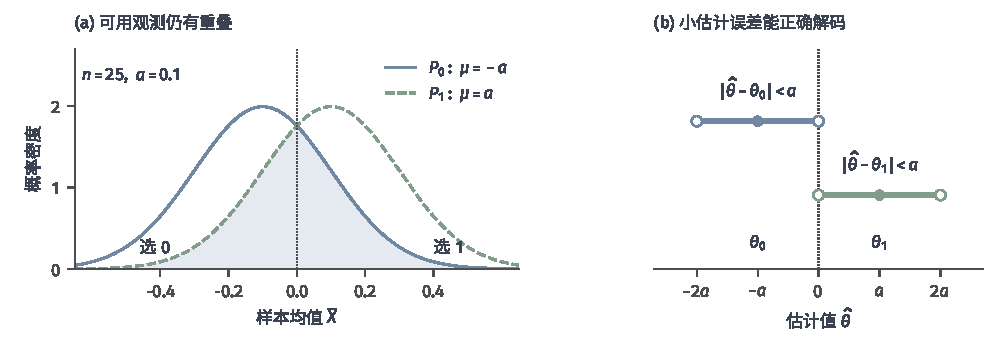
\includegraphics[width=169mm]{figures/00-shared/mathematical-preliminaries-lower/01-random-variables-distributions-and-causality/matplotlib/information-le-cam-estimation-testing/figure.pdf}
  \caption{由估计精度连接到二选一检验的高斯教学例。取\(\sigma=1,n=25,a=0.1\)，左图样本均值在两候选下分别服从\(\mathcal N(-a,0.2^2)\)与\(\mathcal N(a,0.2^2)\)；浅蓝阴影是两密度逐点较小值之下的面积，等于\(1-d_{\mathrm{TV}}\)，其一半约为\(0.3085\)，是最小等先验总体错误。右图的实点为目标，空心端点不属于对应的开误差区间；两个区间只在边界处相接。正文的\(1/4\)是经Pinsker放缩得到的下界，并非左图的精确最小错误。}
  \label{fig:information-le-cam-estimation-testing}
\end{figure*}

\subsubsection{多个候选的区分下界}
\label{sec:information-many-candidates}

两点只要求区分一个二元选择；高维问题可能同时包含许多不同目标。
令\(V\)在\(\{1,\ldots,M\}\)上均匀，给定\(V=v\)后观测\(Z\sim P_v\)。
解码器\(\widehat V(Z)\)的错误概率记为\(p_{\mathrm e}\)。
即使\(Z\)连续，\(V\)的条件熵仍可按其有限后验概率求熵，再对\(Z\)积分。

\begin{theorem}[Fano不等式]
\label{thm:information-fano}
对\(M\geq2\)及上述观测模型，
\begin{equation}
  p_{\mathrm e}\geq1-\frac{I(V;Z)+\log2}{\log M}.
  \label{eq:information-fano}
\end{equation}
\end{theorem}
\begin{proof}
令\(E=\mathbb I\{\widehat V\neq V\}\)。给定\(Z\)且\(E=0\)时，
\(V=\widehat V(Z)\)已确定；给定\(E=1\)时，至多还有\(M-1\)个可能索引。
有限字母表上最大熵为均匀熵，这也可由与均匀分布的Gibbs不等式得到。
于是
\[
\begin{aligned}
  H(V\mid Z)
  &\leq H(V,E\mid Z)\\
  &=H(E\mid Z)+H(V\mid E,Z)\\
  &\leq\log2+p_{\mathrm e}\log(M-1)
   \leq\log2+p_{\mathrm e}\log M.
\end{aligned}
\]
又因\(H(V)=\log M\)，互信息分解给出
\(H(V\mid Z)=\log M-I(V;Z)\)。移项得到结论。
随机化解码可把独立随机种子并入\(Z\)，不会增加关于\(V\)的信息。
\end{proof}

若目标集合中有两两距离至少\(2s\)的有限分离集
\(\{\theta_1,\ldots,\theta_M\}\)，误差小于\(s\)就能最近邻解码。
这把前面计数与打包的工具接到统计下界：候选多能提高\(\log M\)，
但必须同时控制观测中含有多少索引信息\scite{math-cover2006information}
令\(\overline P=M^{-1}\sum_uP_u\)，则
\[
  I(V;Z)=\frac1M\sum_vD_{\mathrm{KL}}(P_v\Vert\overline P)
  \leq\frac1{M^2}\sum_{v,u}D_{\mathrm{KL}}(P_v\Vert P_u).
\]
等式来自给定\(V\)的条件KL分解；不等式来自
\(-\log(M^{-1}\sum_u p_u)\leq M^{-1}\sum_u(-\log p_u)\)。
因此
\(\max_vP_v\{d(\widehat\theta,\theta_v)\geq s\}\)
至少为Fano右侧，若右侧为负则只得到平凡下界零。

保留一个可复算的四候选构造：均值为\(\{-3a,-a,a,3a\}\)，
每个候选产生\(n\)个方差\(\sigma^2\)的独立高斯观测。
最小间距为\(2a\)，有序候选对的平均平方距离为\(10a^2\)，故
\[
  I(V;Z)\leq\frac{5na^2}{\sigma^2}.
\]
取\(a=\sigma/(4\sqrt n)\)时右侧为\(5/16\)，Fano给出
\(p_{\mathrm e}\geq1-(5/16+\log2)/\log4\approx0.2746\)。
任意估计器因此至少在一个候选上以这一概率产生不小于\(a\)的误差。
目标分离与观测接近必须同时成立；只罗列许多模型不构成下界证明。

\subsection{序贯观测下的分布区分}
\label{sec:information-sequential-observations}

若观测位置根据已获得的结果改变，最终资料的联合分布也随算法改变。
仍可使用前面的检验不等式，但比较对象应当是包含行动与结果的完整轨迹。

\subsubsection{重复与时序观测的信息累积}
\label{sec:information-sequential-accumulation}

独立重复是简单情形。固定有限个分量\(t=1,\ldots,T\)，假设\(P_t\ll Q_t\)，密度比为\(L_t\)。
乘积规律的比值为\(\prod_tL_t\)，因此
\[
\begin{aligned}
  D_{\mathrm{KL}}\left(\bigotimes_tP_t\Big\Vert\bigotimes_tQ_t\right)
     &=\sum_tD_{\mathrm{KL}}(P_t\Vert Q_t),\\
  D_\alpha\left(\bigotimes_tP_t\Big\Vert\bigotimes_tQ_t\right)
     &=\sum_tD_\alpha(P_t\Vert Q_t),\qquad\alpha>1.
\end{aligned}
\]
第一式由对数把乘积化为和；第二式由独立性使
\(\mathbb E_{\otimes Q_t}\prod_tL_t^\alpha=\prod_t\mathbb E_{Q_t}L_t^\alpha\)。
公式可按扩展值理解，不通过相减处理无限项。

一般序列不独立。设\(Z_{0:T}\)在标准Borel空间取值，两个规律分解为初始分布及
历史条件核，\(P_0\ll Q_0\)，且在相关的\(P\)-历史上
\(P_t(\cdot\mid Z_{<t})\ll Q_t(\cdot\mid Z_{<t})\)。
\BookChapterRef{chap:random-sequences-and-processes}{第~\ref{chap:random-sequences-and-processes}章}的轨迹换测度给出联合密度比
\[
  L_{0:T}=L_0(Z_0)\prod_{t=1}^T L_t(Z_t\mid Z_{<t}).
\]
对数相加，再对每一项先按历史条件平均，得到
\begin{equation}
\begin{aligned}
 D_{\mathrm{KL}}(P_{0:T}\Vert Q_{0:T})
 &=D_{\mathrm{KL}}(P_0\Vert Q_0)\\
 &\quad+\sum_{t=1}^T\mathbb E_{Z_{<t}\sim P}
 D_{\mathrm{KL}}\bigl(P_t(\cdot\mid Z_{<t})
                     \Vert Q_t(\cdot\mid Z_{<t})\bigr).
\end{aligned}
\label{eq:information-trajectory-kl-chain}
\end{equation}
这是式~\eqref{eq:information-kl-conditional-chain}的反复应用。
有限时域中每个条件对数比的负部积分均有统一有限界，
故可合法按扩展值累加；得到有限数值则还需累计条件KL有限。
期望必须沿前向分布\(P\)实际产生的历史计算。

轨迹包含行动时，同一算法在同一历史上使用相同的条件行动核，
所以比较两个环境时行动因子相消；两个环境的历史频率却不会相消。
在同一环境比较两条策略时，则是环境核相消，剩下条件行动KL。
若两者都改变，不能省略其中任何一组项。

Rényi不能把条件散度直接按\(P\)平均。一个充分组合条件是：在\(Q\)-几乎处处的历史上，
\(P_t(\cdot\mid h_{<t})\ll Q_t(\cdot\mid h_{<t})\)，并且有确定的统一界
\[
  D_\alpha(P_t(\cdot\mid h_{<t})\Vert Q_t(\cdot\mid h_{<t}))
  \leq\varepsilon_t.
\]
为简化记号从\(t=1\)开始且初始历史固定。在\(Q\)下从最后一步取条件期望，
\[
  \mathbb E_Q[L_t^\alpha\mid h_{<t}]
       \leq e^{(\alpha-1)\varepsilon_t}.
\]
前面的密度比是历史可测量，因此每消去一步至多乘上这个常数。
反复迭代后
\[
  \mathbb E_Q L_{1:T}^{\alpha}
  \leq e^{(\alpha-1)\sum_t\varepsilon_t},\qquad
  D_\alpha(P_{1:T}\Vert Q_{1:T})\leq\sum_t\varepsilon_t.
\]
若只在某种历史分布下给出平均条件界，后续选择可能偏向高散度历史，
不能据此使用这个组合结论。

固定有限时域无需停止论证。若共同停止规则给出\(\tau\leq T\)，
停止后补同一个吸收符号，其条件信息代价为零，公式仍适用。
无界停时则应确认在所比较的规律下几乎处处终止；
一种足够的取极限条件是截断累计对数似然比
\(\log L_{0:\tau\wedge n}\)在\(P\)下均匀可积并收敛到停止轨迹的对数密度比。
此时左侧期望可取极限，右侧的非负条件KL用单调收敛。
终止本身不能代替这些可积条件。
隐私分析若使用组合式，还必须另外规定相邻输入、随机机制，
以及对全部相邻输入统一成立的界；单个分布对的散度不是完整隐私定义。

\subsubsection{自适应观测的区分下界}
\label{sec:information-adaptive-lower-bounds}

固定有限时域\(T\)，设算法\(\mathcal A\)在时刻\(t\)根据历史，
从有限或可数位置集合中选择来源或状态行动对\((s,a)\)。
观测取值于标准Borel空间，在环境\(j\)中的核为\(P_j(\cdot\mid s,a)\)，
并假设每个允许位置上都有\(P_0(\cdot\mid s,a)\ll P_1(\cdot\mid s,a)\)。
若初始规律相同、条件行动规则相同，且观测在给定历史及当前\((s,a)\)后使用该核，
轨迹链式法则可按访问位置分组：
\[
  D_{\mathrm{KL}}(\mathbb P_0^{\mathcal A}\Vert\mathbb P_1^{\mathcal A})
  =\sum_{s,a}\mathbb E_0N_T(s,a)\,
      D_{\mathrm{KL}}(P_0(\cdot\mid s,a)\Vert P_1(\cdot\mid s,a)).
\]
这里\(N_T(s,a)\)为\(T\)步中的访问次数；等式来自
\(\sum_t\mathbb I\{(S_t,A_t)=(s,a)\}=N_T(s,a)\)。
当某位置的期望访问次数为零时，该项约定为零，即使位置核的KL为无限。
访问次数是由算法和环境共同产生的随机量，不能预先替换成均匀独立的样本数。
连续位置不能用点访问次数的可数求和表示；此时应保留式~\eqref{eq:information-trajectory-kl-chain}
中的逐时条件期望，或对期望访问测度积分。
核若还依赖其他历史，保留逐步条件KL形式，不能强行按固定位置常数提取。

考虑两个可选Bernoulli来源\(A,B\)。环境\(0\)的均值为
\((1/2+\varepsilon,1/2)\)，环境\(1\)为
\((1/2+\varepsilon,1/2+2\varepsilon)\)，\(0<\varepsilon<1/4\)。
每次访问给出独立于过去的相应来源新观测，但来源选择允许自适应。
两个环境的最优来源相反，全部区分信息只来自\(B\)，单次KL为
\[
  \kappa(\varepsilon)
  =D_{\mathrm{KL}}\bigl(\operatorname{Bernoulli}(1/2)
             \Vert\operatorname{Bernoulli}(1/2+2\varepsilon)\bigr)
  =-\tfrac12\log(1-16\varepsilon^2).
\]
故轨迹KL为\(\mathbb E_0N_T(B)\kappa(\varepsilon)\)。
若输出的来源在两个环境下的错误都不超过\(\delta<1/2\)，
检验恒等式迫使TV至少为\(1-2\delta\)，Pinsker进一步给出
\[
  \mathbb E_0N_T(B)\geq
  \frac{2(1-2\delta)^2}{\kappa(\varepsilon)}.
\]
例如\(\varepsilon=0.1,\delta=0.1\)，有
\(\kappa\approx0.08718\)，期望访问至少约\(14.68\)次。
当\(\varepsilon\)小时，\(\kappa=8\varepsilon^2+O(\varepsilon^4)\)，
因此固定错误水平需要\(\varepsilon^{-2}\)量级的区分观测。
这是信息不足的预算下界，不是某个算法已达到该预算的上界。
推广到无界停止必须满足上一段的终止和可积条件；
更具体的价值或累计决策损失还要引入相应任务定义。

\section{候选模型的比较与总体评价}
\label{sec:stats-model-comparison-data-acquisition}
\subsection{模型证据与信息准则}
\label{sec:statistics-model-evidence}
% Baseline T:1595-1754
在同一观测预算内得到多个候选模型后，还需决定比较的是训练拟合、未来预测还是模型证据。
边缘似然对参数积分，Laplace近似用局部曲率近似这项积分。
信息准则的惩罚形式虽可能相似，比较目标和渐近条件却不同。

\paragraph{预测、似然与边缘似然}
模型选择准则并非都在回答同一问题。独立测试误差比较未来预测；训练似然衡量已观测数据
在拟合参数下的密度；边缘似然
\[
  p(\bm y\mid M)
  =\int p(\bm y\mid\vartheta,M)\pi(\vartheta\mid M)\,\mathrm d\vartheta
\]
对参数不确定性积分；编码长度则把模型和数据的描述代价相加。一个模型可能训练似然高，
却因复杂度、先验体积或泛化误差而不被其他准则选择。

\begin{definition}[Bayes因子]
  \label{def:statistics-bayes-factor}
两个模型\(M_1,M_0\)的\term{Bayes因子}（Bayes factor）是
\[
  \operatorname{BF}_{1,0}
  =\frac{p(\bm y\mid M_1)}{p(\bm y\mid M_0)}.
\]
这里两个边缘似然都由概率先验得到；所比较的数据处，分母严格为正且有限，分子有限且可为零。
\end{definition}
Bayes因子更新的是模型间先验赔率，
不是与先验无关的“模型为真概率”。在高斯位置模型中，若
\(\theta\sim\mathcal N(0,A^2)\)，则
\(\overline Y\sim\mathcal N(0,A^2+\sigma^2/n)\)。保持似然峰值不变而增大\(A\)
会把先验质量摊到更宽区域；对固定\(\overline y\)，当\(A\to\infty\)时该边缘密度
趋于零。这正是模型证据依赖参数先验尺度的一个可复核例子。

\paragraph{Laplace近似与BIC}
边缘似然需要对全部参数积分，不能只取最大似然值。若样本增加后积分集中在一个内部峰值附近，就可用峰值处的二阶展开把形状近似为高斯：峰高记录拟合，曲率记录高密度区域的宽度，先验记录该区域原先获得的权重。下面的尾部条件用于保证峰外贡献确实可忽略。
\begin{theorem}[固定维Laplace局部积分近似]
\label{thm:statistics-laplace-approximation}
设\(\Theta\subseteq\mathbb{R}^d\)为可测集，
\(\widehat{\bm\vartheta}\in\operatorname{int}(\Theta)\)。函数
\(h:\Theta\to\mathbb{R}\)可测，并在
\(\widehat{\bm\vartheta}\)的某个邻域内二阶连续可微；该点是\(h\)在\(\Theta\)上的
唯一全局最大点，且
\(\bm H=-\nabla^2h(\widehat{\bm\vartheta})\)正定。函数
\(g:\Theta\to[0,\infty)\)局部可积，在该点的某个邻域内连续，并满足
\(g(\widehat{\bm\vartheta})>0\)。

进一步假设存在\(\delta,\eta>0\)和\(n_0\geq1\)，使
\(\overline{B_\delta(\widehat{\bm\vartheta})}\subseteq\Theta\)，\(h,g\)在该闭球
所在的邻域内分别满足上述光滑性与连续性，并且
\[
  \sup_{\bm\vartheta\in
    \Theta\setminus B_\delta(\widehat{\bm\vartheta})}
  h(\bm\vartheta)
  \leq h(\widehat{\bm\vartheta})-\eta,
  \qquad
  \int_\Theta
  \exp\!\left\{n_0\bigl[h(\bm\vartheta)
    -h(\widehat{\bm\vartheta})\bigr]\right\}
  g(\bm\vartheta)\,\mathrm d\bm\vartheta<\infty.
\]
则当\(n\to\infty\)时，
\[
  \int_\Theta \exp\{n h(\bm\vartheta)\}g(\bm\vartheta)\,
  \mathrm d\bm\vartheta
  =
  \exp\{nh(\widehat{\bm\vartheta})\}
  g(\widehat{\bm\vartheta})
  \left(\frac{2\pi}{n}\right)^{d/2}
  |\bm H|^{-1/2}\{1+o(1)\}.
\]
\end{theorem}

\begin{proof}
正定性与二阶连续性保证：必要时缩小\(\delta\)，存在\(c>0\)，使闭球内有
\[
  h(\bm\vartheta)-h(\widehat{\bm\vartheta})
  \leq-c\lVert\bm\vartheta-\widehat{\bm\vartheta}\rVert_2^2.
\]
缩小闭球后，原闭球中剩余的紧致环带由唯一最大性给出严格间隔；把它与原来的尾部间隔
合并，仍可取某个\(\eta>0\)满足定理中的一致上界。另一方面，在最大点附近作多元
Taylor展开：
\[
  h(\bm\vartheta)
  =
  h(\widehat{\bm\vartheta})
  -\frac12(\bm\vartheta-\widehat{\bm\vartheta})^\top
  \bm H(\bm\vartheta-\widehat{\bm\vartheta})
  +o(\lVert\bm\vartheta-\widehat{\bm\vartheta}\rVert_2^2).
\]
令
\(\bm u=\sqrt n\,\bm H^{1/2}
(\bm\vartheta-\widehat{\bm\vartheta})\)，则逆变换的Jacobian行列式绝对值为
\(n^{-d/2}|\bm H|^{-1/2}\)，即
\(\mathrm d\bm\vartheta
=n^{-d/2}|\bm H|^{-1/2}\mathrm d\bm u\)。对每个固定的\(\bm u\)，
Taylor展开与\(g\)的连续性
使变换后的被积函数收敛到
\(g(\widehat{\bm\vartheta})\exp(-\lVert\bm u\rVert_2^2/2)\)。局部二次上界和
\(g\)在闭球上的有界性给出可积的高斯控制函数，因此支配收敛定理给出
\[
\begin{aligned}
  &\int_{B_\delta(\widehat{\bm\vartheta})}
  \exp\!\left\{n\bigl[h(\bm\vartheta)
    -h(\widehat{\bm\vartheta})\bigr]\right\}
  g(\bm\vartheta)\,\mathrm d\bm\vartheta\\
  &\qquad=n^{-d/2}|\bm H|^{-1/2}
  g(\widehat{\bm\vartheta})(2\pi)^{d/2}\{1+o(1)\}.
\end{aligned}
\]
闭球外的尾项满足
\[
\begin{aligned}
  &\int_{\Theta\setminus B_\delta(\widehat{\bm\vartheta})}
  e^{n[h(\bm\vartheta)-h(\widehat{\bm\vartheta})]}
  g(\bm\vartheta)\,\mathrm d\bm\vartheta\\
  &\qquad\leq e^{-(n-n_0)\eta}
  \int_\Theta
  e^{n_0[h(\bm\vartheta)-h(\widehat{\bm\vartheta})]}
  g(\bm\vartheta)\,\mathrm d\bm\vartheta\\
  &\qquad=o(n^{-d/2}).
\end{aligned}
\]
局部主项与该尾项相加即得结论。
\end{proof}

上一定理描述固定函数\(h\)的基本形式。在正则独立样本模型中，实际处理的是随机函数
序列
\[
  nh_n(\bm\vartheta)=\ell_n(\bm\vartheta)
  =\sum_{i=1}^n\log p_\vartheta(y_i),\qquad
  g(\bm\vartheta)=\pi(\bm\vartheta).
\]
若极大似然估计以内点唯一最大点的形式收敛，归一化观测信息矩阵收敛到正定极限，先验
在极限点附近连续且为正，并且局部二次展开与尾部控制对该序列一致成立，则相同论证给出
\[
  \log p(\bm y\mid M)
  =
  \ell_n(\widehat{\bm\vartheta})
  -\frac d2\log n+O_{\mathbb{P}}(1).
\]
对固定的有限候选模型集合，乘以\(-2\)并只保留随\(n\)发散的项，得到常用形式
\[
  \operatorname{BIC}
  =-2\ell_n(\widehat{\bm\vartheta})+d\log n.
\]
惩罚来自后验高密度区域体积随\(n^{-d/2}\)缩小，而不是人为给参数个数加价。

\paragraph{AIC、描述长度与比较口径}
在独立、固定维且正则的最大似然设定中，常用
\[
  \operatorname{AIC}
  =-2\ell_n(\widehat{\bm\vartheta})+2d.
\]
其中\(2d\)是一阶校正拟合对预期样本外对数损失的乐观偏差，目标是预测失配；模型失配
时还要核对适用的协方差校正，不能只数参数。BIC近似特定先验下的边缘似然，常以候选中
存在真模型的正则渐近为背景。\term{最小描述长度}（minimum description length,
MDL）则先规定可解码的模型代码与给定模型后的数据代码，再最小化二者总长度；更换编码
对象或精度约定会改变有限样本准则。三者惩罚形式相似时也不能互换解释，更不能共享未经
证明的选择一致性。

混合模型的标签交换、参数位于边界、额外成分权重为零或Fisher信息奇异时，最大点可能
不唯一，局部曲率可能退化，常规Laplace展开和\(d\log n\)惩罚随之失效。此时应使用
适合奇异模型的方法、数值积分或明确的近似；近似边缘似然不能写成精确证据。

\subsection{独立评价与交叉验证}
\label{sec:statistics-validation-pipeline}
% Baseline T:1294-1326
候选越多，偶然低估越容易被选中。解决办法是把选择和最终评价分开，或把“选择算法”
整体作为待评价对象。固定模型的区间不能在选择后继续冒充选中模型的区间。

例~\ref{ex:statistics-running-sensor-calibration}还需要从两个预先给定的带宽中选择一个。
用一个刻意简化、可精确计算的噪声模型说明选择偏差：假设两个带宽的真实预测均方误差都
是\(4\)，验证误差分别为
\[
  \widehat R_j=4+\varepsilon_j,\qquad
  \mathbb{P}(\varepsilon_j=0.8)
  =\mathbb{P}(\varepsilon_j=-0.8)=\frac12,
  \quad j=1,2,
\]
并且两个误差独立。每个\(\widehat R_j\)单独都是无偏的，但两者最小值以概率
\(1/4\)等于\(4.8\)，以概率\(3/4\)等于\(3.2\)，所以
\[
  \mathbb{E}\min(\widehat R_1,\widehat R_2)
  =\frac14\times4.8+\frac34\times3.2
  =3.6.
\]
所报告的最小验证误差平均为\(3.6\)，低于选中带宽的真实风险\(4\)，平均低估\(0.4\)。嵌套交叉验证或独立测试集的
作用，是评价“比较两个带宽再选择”这一完整流程，而不是重新评价已知固定的单个带宽。

\paragraph{交叉验证与流程评价}
\term{交叉验证}（cross-validation）把数据轮流分成训练部分和验证部分，估计“用同样
训练流程在新数据上的预测误差”。它同时依赖训练规模、划分单位和调参流程。若用同一组
折选择超参数又报告最优分数，结果仍含选择乐观偏差；需要嵌套交叉验证或独立测试集评估
整个选择流程。

交叉验证各折的误差通常相关，因为训练集大量重叠，不能默认它们独立。因此不能把\(K\)个折分数当成
\(K\)个独立观测，再用普通样本方差构造过窄区间。若目标是比较两个算法，应在相同划分
上计算配对差异，并把数据集抽样和训练随机性纳入评价设计；单次\(K\)折结果主要用于
误差估计与模型选择，不自动提供精确的显著性检验。

\subsection{数据依赖下的总体风险控制}
\label{sec:information-data-dependent-evaluation}

用同一批训练样本既选择模型又评价所选模型，为什么会有问题？打个比方：考完试先让学生看一遍标准答案、挑出自己答对的题，再只报告这些题的正确率，这个分数自然虚高。模型选择相当于让算法看过这批样本后专挑在这批样本上表现好的模型，被选中的模型与这批样本已经产生了依赖，原先“固定模型时样本平均无偏”的结论不再适用。设\(S=(Z_1,\ldots,Z_n)\)独立同分布，学习规则根据\(S\)产生随机训练模型\(W\)。对预先固定的\(w\)，样本损失是独立平均；对选出的\(W\)，模型与样本已经相互依赖。

前面的工具提供两条分析路径。比较真实联合规律与解除依赖的边缘乘积，可以控制平均评价偏差；建立同时覆盖全部候选分布的概率事件，则允许看过样本以后选择候选。两条路径的目标和量词不同：对重复抽取训练集所得误差的平均控制，不能替代对一批随机训练样本以高概率成立的误差界。

\subsubsection{数据依赖下的平均评价偏差}
\label{sec:information-mi-generalization}

设可测损失\(\ell(w,Z)\in[0,1]\)，新样本\(Z\)服从与训练样本相同的总体规律，
定义
\[
  \begin{aligned}
    R(w)&=\mathbb E_Z\ell(w,Z),&
    \widehat R_S(w)&=\frac1n\sum_{i=1}^n\ell(w,Z_i),\\
    g(S,w)&=R(w)-\widehat R_S(w).
  \end{aligned}
\]
固定\(w\)时，\(\mathbb E_Sg(S,w)=0\)。
Hoeffding引理对每个中心化损失给出指数矩，再用独立性相乘，有
\[
  \mathbb E_Se^{t g(S,w)}\leq e^{t^2/(8n)},\qquad t\in\mathbb R.
\]
界不依赖\(w\)。在边缘乘积\(Q=P_S\otimes P_W\)下再对\(w\)积分，
因此\(\mathbb E_Qg=0\)，且\(g\)的方差代理为\(1/(4n)\)。
真实评价使用联合分布\(P=P_{S,W}\)，换测度的代价正是
\[
  D_{\mathrm{KL}}(P\Vert Q)=I(S;W).
\]
若互信息有限，式~\eqref{eq:information-subgaussian-change-measure}给出
\begin{equation}
  \left|\mathbb E_{S,W}\{R(W)-\widehat R_S(W)\}\right|
  \leq\sqrt{\frac{I(S;W)}{2n}}.
  \label{eq:information-mi-generalization}
\end{equation}
无限互信息时右侧无限，不提供有效保证。
这是平均有符号泛化差的绝对值，并不是
\(\mathbb E|R(W)-\widehat R_S(W)|\)，也没有给出
\(|R(W)-\widehat R_S(W)|\)以高概率不超过某个阈值的保证。

例如算法只能输出\(M\)种预测器，则\(I(S;W)\leq H(W)\leq\log M\)，
平均偏差至多\(\sqrt{\log M/(2n)}\)。若算法完全忽略训练样本，互信息为零，
平均有符号差也为零，但每个样本的经验风险仍会波动。
反过来，连续确定性输出可能携带无限互信息；参数维数有限本身不能保证信息有限。
在本节设定中，参与学习与评价的是同一批训练样本，因此控制量是训练模型对这批样本的依赖。若改用独立评价样本，应按新的联合规律重新计算互信息；参数个数不能代替这种依赖。

\subsubsection{数据依赖下的同时风险控制}
\label{sec:information-pac-bayes}

上一条互信息界控制重复抽取训练样本时的平均偏差，不直接保证一次随机训练样本上的风险差以高概率很小。现在允许学习规则根据训练样本\(S\)给出候选模型上的分布\(Q_S\)，并考察先抽取\(w\sim Q_S\)、再用该候选预测所得到的平均总体风险\(\mathbb E_{Q_S}R(w)\)。它不同于先平均各候选的预测值、再评价聚合预测器的风险。例如两个常值预测\(-1,1\)在真实值\(0\)处的平方损失均为\(1\)，等权抽取候选后的平均损失为\(1\)，先平均预测却得到\(0\)、损失也为\(0\)。投票或平均集成需要另行给出聚合规则，不能直接把本节的平均候选风险当成其风险。

为了覆盖依据训练样本选择的\(Q_S\)，先建立对全部允许候选分布同时成立的高概率事件。PAC--Bayes界以观察\(S\)前固定的\(P_0\)为参考，用\(D_{\mathrm{KL}}(Q_S\Vert P_0)\)度量候选分布相对参考的偏离。\(P_0\)与\(Q_S\)均定义在前文以\(w\)索引的模型空间上；这个参考先验用于风险证明，不要求来自贝叶斯生成模型。下述调节参数\(\lambda\)与先验都须在观察这批评价所用的训练样本前确定。

\begin{theorem}[固定参数的基础PAC--Bayes界]
\label{thm:information-pac-bayes-basic}
在上述独立同分布样本和\([0,1]\)损失设定下，令\(P_0\)在观察\(S\)前固定，
且与\(S\)独立。对任意预先固定的\(\lambda>0\)与\(0<\delta<1\)，
以至少\(1-\delta\)的概率，同时对所有\(Q\ll P_0\)有
\begin{equation}
  \mathbb E_QR(w)
  \leq\mathbb E_Q\widehat R_S(w)
  +\frac{D_{\mathrm{KL}}(Q\Vert P_0)+\log(1/\delta)}{\lambda}
  +\frac{\lambda}{8n}.
  \label{eq:information-pac-bayes-basic}
\end{equation}
KL无限时将右侧解释为无限。
\end{theorem}
\begin{proof}
对每个固定\(w\)，Hoeffding引理给出
\(\mathbb E_Se^{\lambda(R(w)-\widehat R_S(w))}
\leq e^{\lambda^2/(8n)}\)。
先验独立于样本，Tonelli定理允许对同一个\(P_0\)平均：
\[
  \mathbb E_S\mathbb E_{w\sim P_0}
  e^{\lambda(R(w)-\widehat R_S(w))}
  \leq e^{\lambda^2/(8n)}.
\]
由Markov不等式，事件
\[
  \mathcal E=
  \left\{S:\mathbb E_{P_0}e^{\lambda(R-\widehat R_S)}
  \leq\frac{e^{\lambda^2/(8n)}}{\delta}\right\}
\]
满足\(P_S(\mathcal E)\geq1-\delta\)。
对任意固定在这个事件内的样本，实现后的函数
\(f(w)=\lambda(R(w)-\widehat R_S(w))\)有界。
对所有\(Q\ll P_0\)分别使用式~\eqref{eq:information-dv-lower}，得到
\[
\begin{aligned}
  \lambda\mathbb E_Q(R-\widehat R_S)
  &\leq D_{\mathrm{KL}}(Q\Vert P_0)
       +\log\mathbb E_{P_0}e^{\lambda(R-\widehat R_S)}\\
  &\leq D_{\mathrm{KL}}(Q\Vert P_0)
       +\frac{\lambda^2}{8n}+\log(1/\delta).
\end{aligned}
\]
除以\(\lambda\)即得所需结论。事件只包含先验积分，不随\(Q\)改变，
因此在事件发生后选择的数据依赖\(Q_S\)也被同时覆盖。
\end{proof}

若\(P_0\)均匀分布在预先指定的\(M\)个候选上，
选择其中一个候选的点质量\(Q\)具有KL为\(\log M\)，
便得到这\(M\)个预测器的统一风险控制。
若\(P_0\)为连续分布，单点候选通常不对它绝对连续，
不能仍把该点估计作为有限KL的候选代入。

“固定\(\lambda\)”是事件成立的条件。观察数据后逐个候选优化右侧的
\(\lambda\)，或根据同一评价样本重选先验，都超出了上述事件。
可以预设可数参数网格并分配失败概率后使用并集界，
也可以用独立样本确定先验，再对剩余评价样本条件化应用定理。
这些额外步骤不能省略。互信息界比较联合规律与边缘乘积，给出平均偏差；
此处比较候选分布与先验，给出同时风险界，两者复用换测度代数但不是同一个保证。


\section{预算约束下的观测设计}
\label{sec:statistics-design-information}
\subsection{随机比较与重复实验}
% Baseline T:1761-1843
推断质量不仅由分析方法决定，也由数据如何取得决定。每个对象在各处理下本会产生的结果
称为潜在结果，正式的因果目标将在第~\ref{chap:causal-inference}章定义。随机分配使
处理指派在设计上独立于这些预先固定的结果，从而把系统差异转成可量化的随机误差。
配对对照先按对象或关键协变量配对，
再在对内比较。共享噪声以相同加性项进入两项读数时，差值可以消去它；更一般地，正协方差可以降低差值方差。若配对质量差或分析时忽略配对，预期的方差收益不会自动
出现。

先看最简单的两组位置模型。若随机分配后两组分别有\(n_A,n_B\)个独立观测，均值为
\(\mu_A,\mu_B\)，方差为\(\sigma_A^2,\sigma_B^2\)，则
\[
  \widehat\Delta=\overline Y_A-\overline Y_B,\qquad
  \mathbb{E}[\widehat\Delta]=\mu_A-\mu_B,
\]
\[
  \operatorname{Var}(\widehat\Delta)
  =\frac{\sigma_A^2}{n_A}+\frac{\sigma_B^2}{n_B}.
\]
随机化建立的是处理指派与处理前对象特征之间的概率关系，并不要求两种处理下的结果
服从同一分布。上式还假设组间独立且组内方差有限；配对随机化应改为分析对内差值。
它提供的是设计下的可复核比较，潜在结果目标及从试验人群向目标总体的推广条件由
第~\ref{chap:causal-inference}章继续建立。

消融实验删除一个组件并保持其他条件不变，用来判断该组件对整体结果的增量贡献。它不能
在组件强交互时给出唯一的“独立贡献”，也不能用不同训练预算的两个系统冒充单因素比较。
基线、随机种子、停止规则和评价集都应在比较前固定。

学习曲线把训练样本量或计算量与验证性能联系起来。只报告最终点无法区分方法是数据效率
更高，还是只是使用了更多数据和算力。实验至少要区分数据预算、计算预算与评价时间预算：
收集更多标签、搜索更多配置和反复占用测试集是三种不同资源。

\subsection{精度目标下的样本分配}
预算分配应对应希望降低的误差。设\(\sigma_A,\sigma_B>0\)，先把样本量看作正的连续变量。若两组单位观测成本相同且
\(n_A+n_B=N\)，最小化上面的均值差方差可得
\[
  \frac{n_A}{n_B}=\frac{\sigma_A}{\sigma_B}.
\]
这是对\(n_A\)求导或用Cauchy--Schwarz得到的Neyman分配：波动较大的组需要更多
观测。方差未知时要用先验信息或先导样本估计，估计误差也应计入设计；整数、最低组规模
和不同成本会改变解。

线性观测模型
\(\bm y=\bm X\bm\beta+\bm\varepsilon\)提供了多方向设计的接口，其中
\(\bm X\in\mathbb{R}^{n\times d}\)、\(\bm\beta,\bm a\in\mathbb{R}^d\)。
给定满列秩设计矩阵\(\bm X\)，假设
\(\mathbb{E}[\bm\varepsilon\mid\bm X]=\bm{0}\)且
\(\operatorname{Cov}(\bm\varepsilon\mid\bm X)=\sigma^2\bm I_n\)。
普通最小二乘估计量为
\[
  \widehat{\bm\beta}
  =(\bm X^\top\bm X)^{-1}\bm X^\top\bm y.
\]
它在给定\(\bm X\)时无偏，并且
\[
  \operatorname{Var}(\bm a^\top\widehat{\bm\beta}\mid\bm X)
  =\sigma^2\bm a^\top(\bm X^\top\bm X)^{-1}\bm a.
\]
因此新增观测的特征方向会改变设计矩阵，并降低某些\(\bm a\)方向的方差；它未必同样
改善其他方向、预测总体或非线性目标。最小化最坏方向、平均方向或行列式体积会得到不同
设计准则，必须先声明评价对象。

\subsection{信息价值与自适应查询}
当标注预算有限时，\term{主动学习}（active learning）根据当前模型选择下一批待标注
样本。若效用\(U\)已经包含任务收益与查询成本，一个理想选择可写成最大化期望效用增量：
\[
  x^\star\in\argmax_x
  \mathbb{E}_{Y\mid x,\mathcal D}
  \left[
    U(\mathcal D\cup\{(x,Y)\})-U(\mathcal D)
  \right],
\]
其中\(U\)衡量后验不确定性减少或决策效用增加。只选当前最不确定样本是一种替代规则，
不一定等于任务价值最大。如果当前后验熵与查询后的期望后验熵都有限，就可以把效用设为后验熵的负值，即\(U(\mathcal D)=-H(\Theta\mid\mathcal D)\)，此时期望效用增量正是预期熵下降，才与
第~\ref{chap:information-theory-and-statistical-geometry}章的互信息接口相连；若
改按决策风险评价，记
\[
 r(\mathcal D)=\inf_a\mathbb E[\ell(a,\Theta)\mid\mathcal D],
 \qquad U(\mathcal D)=-r(\mathcal D).
\]
这里取有限的最优风险并使用其负值作效用，期望增量才是风险的下降：
\[
 r(\mathcal D)-
 \mathbb E_{Y\mid x,\mathcal D}r(\mathcal D\cup\{(x,Y)\}).
\]
若一次查询还有成本，就从这项下降中扣除该成本，不再重复计入效用。
这接到\BookSectionRef{sec:decision-value-of-information}{第~\ref{sec:decision-value-of-information}节}的信息价值。
信息量增加与任务效用增加不是同一命题。

主动选择会改变被标注样本的分布。若候选池不覆盖目标总体，算法无法询问缺失区域；
若标注噪声随难度变化，不确定样本还可能最不可靠；若最终指标用同一批自适应选择数据
计算，评价也会偏移。因此应在比较前固定可访问数据、查询成本、标注机制和独立评价集。
查询依赖过去答案时，所选特征或对象必须在新噪声揭示前由历史信息确定，才能回用
\BookSectionRef{sec:rv-anytime}{第~\ref{sec:rv-anytime}节}的可预测设计与自适应误差工具；
把自适应记录事后当作固定独立样本没有同样保证。
实验设计不是分析完成后的附注，而是可识别性和误差保证的一部分。

\section{本章小结}
\label{sec:statistics-summary}
有限观测能支持怎样的结论，先由目标、观测机制与可识别性决定。似然、经验准则和后验给出不同的估计方式；缺失、选择、污染与相关性会改变它们所估计的总体以及可用的误差保证。

估计风险、未来预测、参数覆盖和检验错误评价不同对象。渐近效率与信息下界说明精度受到哪些限制，交叉验证和数据依赖风险界则约束选择模型之后怎样解释评价结果。观测设计可以改变信息的来源与数量，但仍需在采集之前明确抽样单位、预算、停止规则和独立评价总体。
